% Completa los datos convenientemente en las zonas marcadas con TODO

\documentclass{beamer}
%PARA VISUALIZAR PRESENTACIONN CON NOTAS USAR VISUALIZADOR "pdfpc":
%Para ver las notas, el cronometro y siguente diapo:
% pdfpc --notes=right slides.pdf
% "tecla p": para pausar el cronometro
\mode<presentation> {
  \usetheme{CambridgeUS}
  \usecolortheme{crane} % color naranja
}
\setbeamercolor{titlelike}{parent=structure,bg=yellow!85!orange} % Cambia el color de la caja del título de la página inicial

\setbeamertemplate{navigation symbols}{} % ocultar iconos de navegación
\setbeamerfont{subsection in toc}{size=\small} % reducir tamaño en TOC
\setbeamerfont{date}{size=\tiny}
\usepackage[spanish]{babel}
\usepackage[utf8]{inputenc}
\usepackage{graphicx}
\usepackage{booktabs}
\usepackage{hyperref}
\usepackage{multicol}
\usepackage{pgfpages}
\usepackage{listings}
\usepackage{multimedia}
\usepackage[export]{adjustbox}
\usepackage{outlines} % Para poner bullets tabulados (\1 \2 \3 ...) y no items

\usepackage{array,tabularx} % para tabular leyenda de ecuaciones
\newenvironment{conditions*} % entorno de "leyenda de ecuación"
  {\par\vspace{\abovedisplayskip}\noindent
   \tabularx{\columnwidth}{>{$}l<{$} @{\ : } >{\raggedright\arraybackslash}X}}
  {\endtabularx\par\vspace{\belowdisplayskip}}
  
% USO DE NOTAS
%\setbeameroption{hide notes} % Para mostrar u ocultar (hide/show)
%\setbeameroption{show only notes} % Mostrar solo las notas
\setbeameroption{show notes on second screen=right} % Mostrar notas en otra pantalla
\setbeamertemplate{note page}{ % asi solo muestro el texto de las notas
  \insertnote%
}

%========= TODO: datos internos del documento
\hypersetup{
	pdftitle={Defensa de trabajo de fin de grado de Ana Martínez Albendea},
	pdfauthor={Ana Martínez Albendea},
	pdfsubject={Sistema inteligente de dispensación y monitorización de
medicamentos para el entorno doméstico},
	pdfkeywords={teaching, robotics, vision, sensors, actuators, ESP32},
	pdfproducer={pdfLaTeX},
  colorlinks=true,
  linkcolor=blue
}
%=========

%========= TODO: diapositiva de portada
\title[MyMeds]{Sistema inteligente de dispensación y monitorización de
medicamentos para el entorno doméstico} % El título reducido aparece en la parte inferior de todas las diapositivas
                                         % El título completo aparece solo en la diapositiva de portada
\author[Ana Martínez Albendea]{Ana Martínez Albendea}
\institute[URJC]
{
\textit{\href{mailto:a.martinezal.2021@alumnos.urjc.es}{\color{blue}{\underline{a.martinezal.2021@alumnos.urjc.es}}}}\\
\vspace{0.5cm}

\includegraphics[width=3cm]{figs/logo-urjc}\\
\vspace{1cm}
Trabajo Fin de Grado
}
\date{16 de julio de 2026}
%=========

%========= COMIENZO DEL DOCUMENTO
\begin{document}

%========= Portada inicial con notas
\begin{frame}[plain] % plain: quita header y footer
\large{\titlepage}
\note[item]{Muchas gracias, buenos días a todos. }
\end{frame}

%========= Licencia
\begin{frame}
\input{licencia.tex}
\end{frame}

%========= Índice o tabla de contenidos (TOC)
\begin{frame}
\frametitle{Contenidos}
%\begin{multicols}{2} % si tengo muchas secciones, lo parte en dos columnas
  \tableofcontents[hideallsubsections] % no muestra subsecciones
%\end{multicols}
\note[item]{Mi nombre es Ana Martínez Albendea y a lo largo de esta presentación explicaré el contexto del proyecto, el diseño y desarrollo del sistema, la validación experimental realizada y, finalmente, las conclusiones obtenidas.}
\end{frame}

%==================================================
\section*{}
\begin{frame}{}
  \centering \Huge
  \emph{Introducción}
\note[item]{Para comenzar, es importante situar este trabajo dentro del ámbito de la robótica de servicios. }
\end{frame}
%==================================================
\section{Introducción}
\subsection{Robótica de servicio}

\begin{frame}
\frametitle{Robótica de servicio}

\begin{figure}
\centering

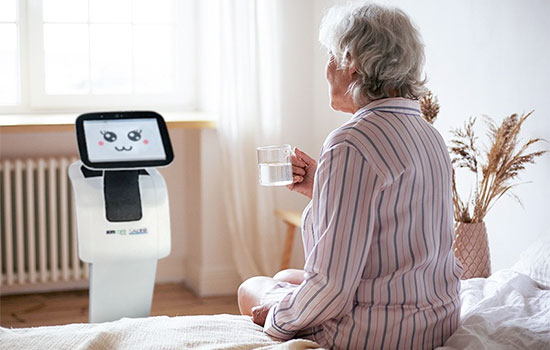
\includegraphics[width=0.44\textwidth,height=3.2cm,valign=c]{figs/robot_asistencial.jpg}
\hspace{0.02\textwidth}
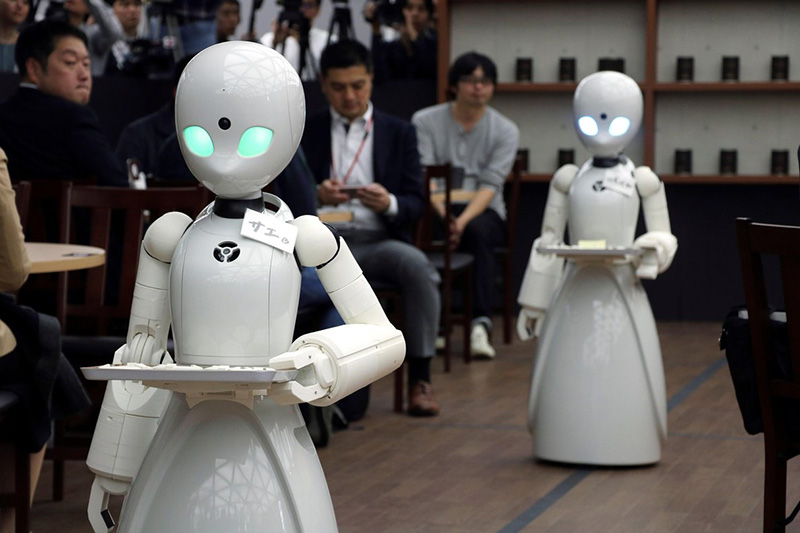
\includegraphics[width=0.44\textwidth,height=3.2cm,valign=c]{figs/Robot_Camarero.jpg}

\vspace{0.3cm}

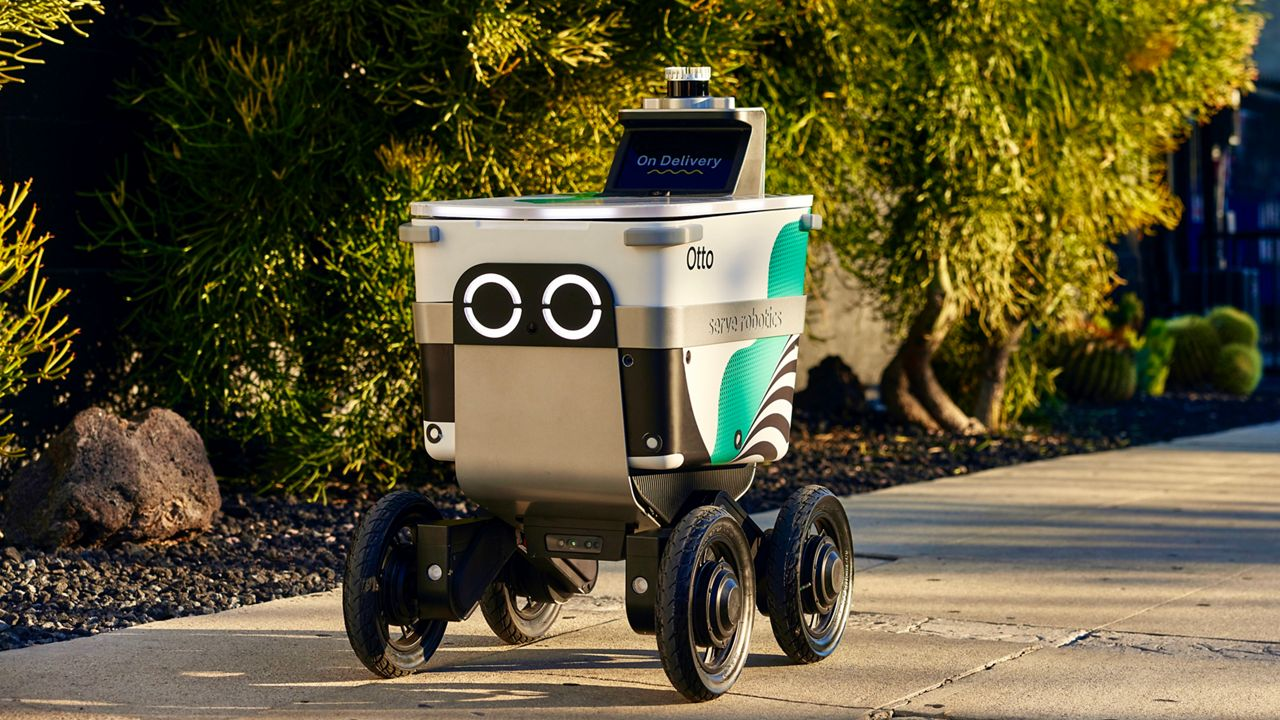
\includegraphics[width=0.44\textwidth,height=3.2cm,valign=c]{figs/Serve_robot.jpeg}
\hspace{0.02\textwidth}

\includegraphics[width=0.44\textwidth,height=3.2cm,valign=c]{figs/stiga.jpg}

\end{figure}

\note[item]{
\item Robótica de servicios
\item Asistencia fuera industria
\item Robótica sanitaria
}


\end{frame}

%==================================================
\subsection{Robótica de asistencia sanitaria}

\begin{frame}
\frametitle{Robótica de asistencia sanitaria}

\begin{figure}
\centering

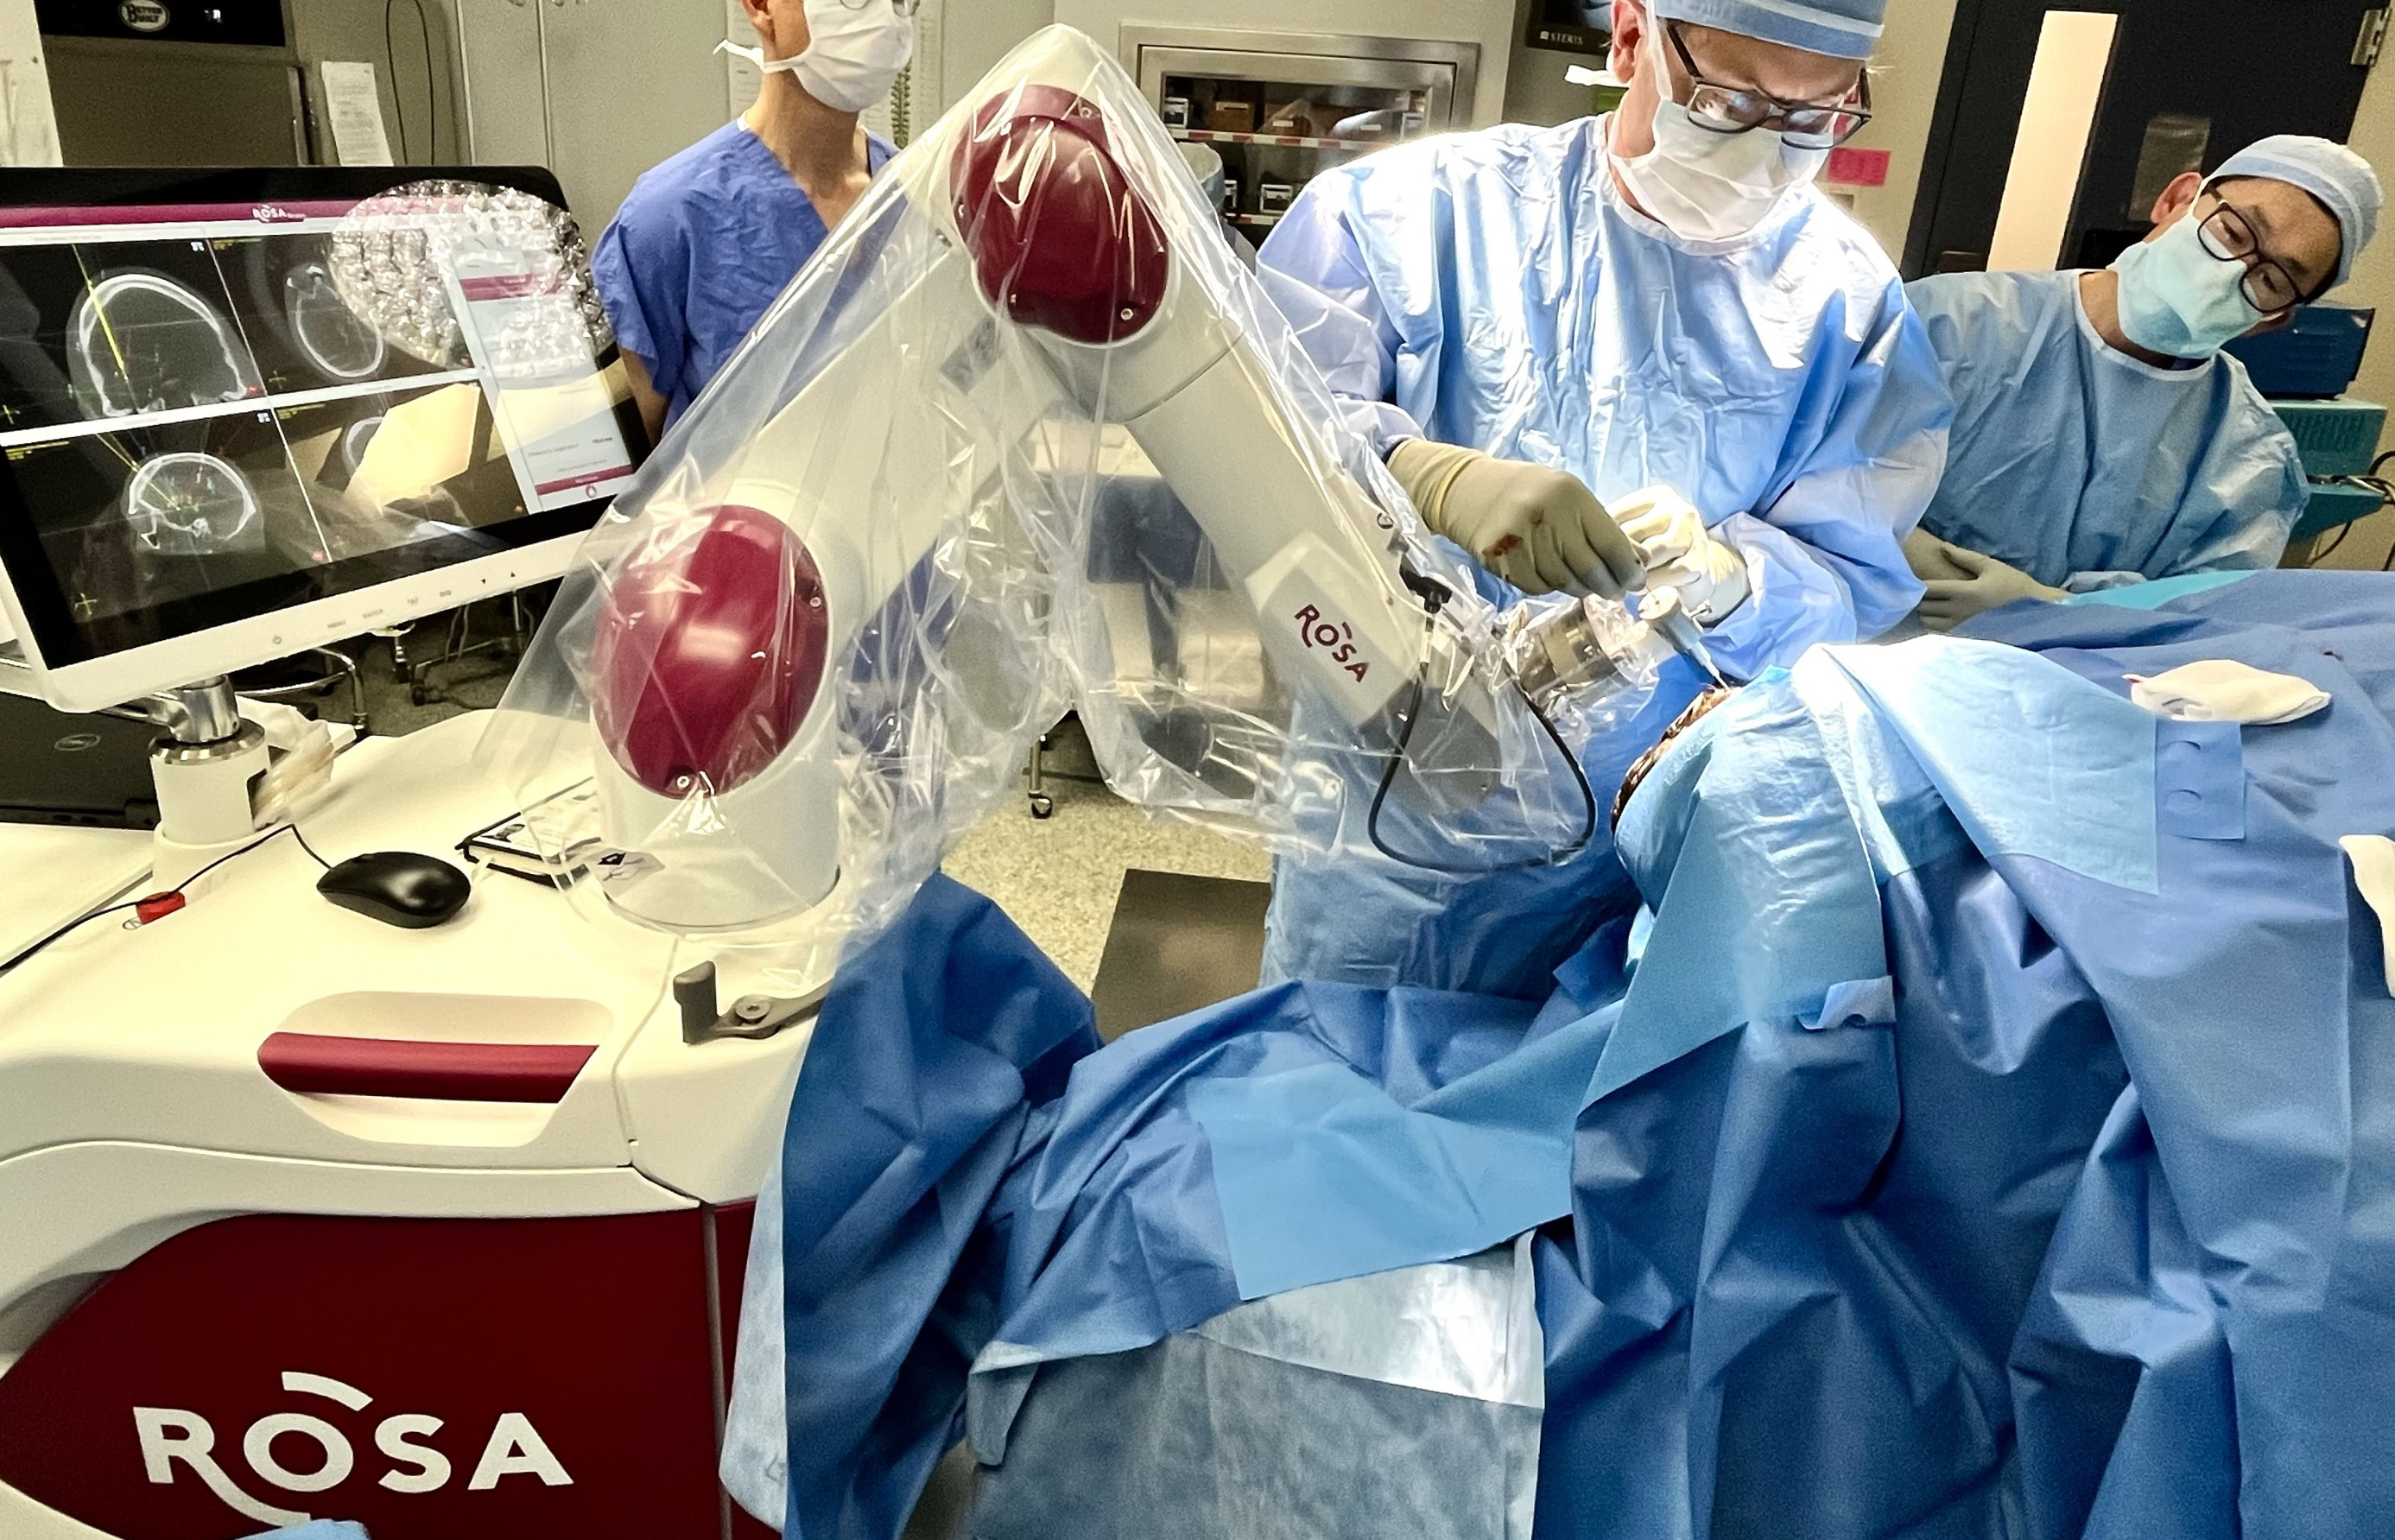
\includegraphics[width=0.445\textwidth,height=3.8cm]{figs/rosa.jpg}
\hspace{0.02\textwidth}
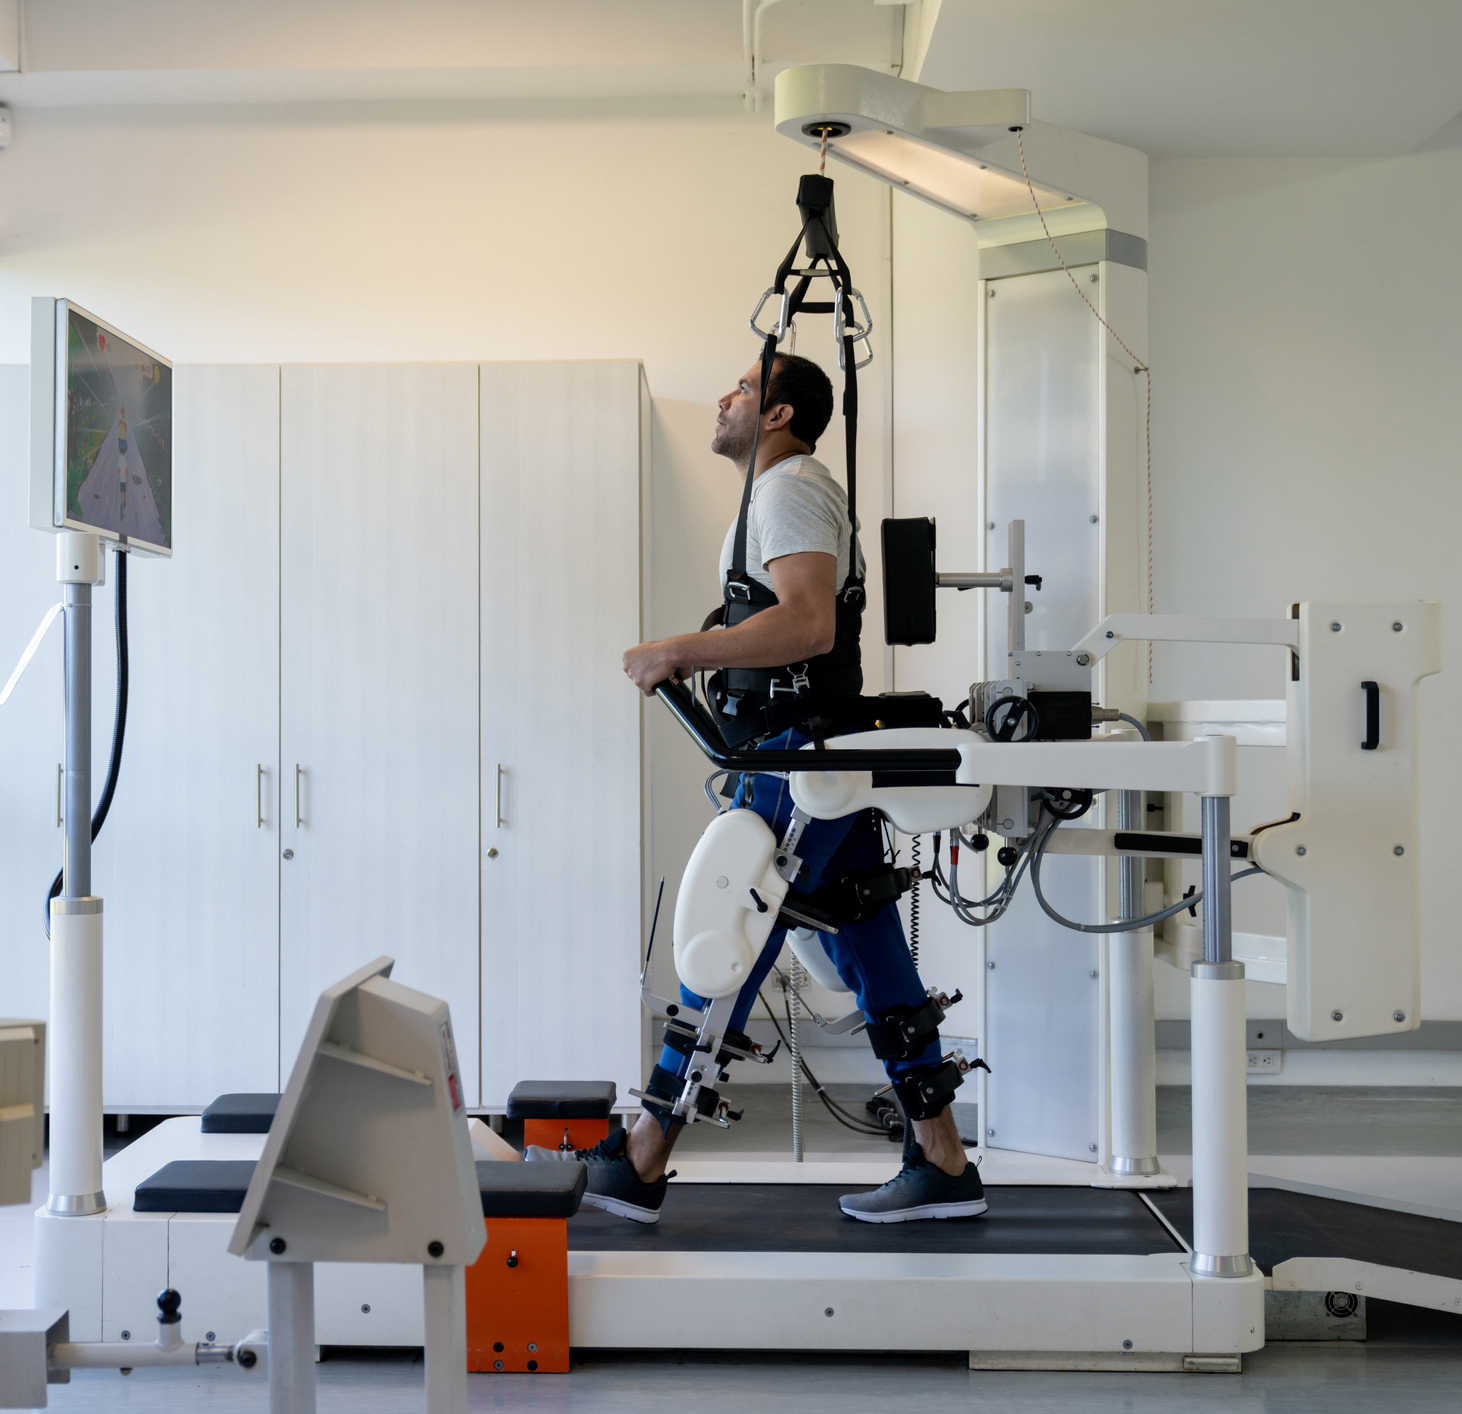
\includegraphics[width=0.445\textwidth,height=3.8cm]{figs/robot_rehab.jpg}

\vspace{0.30cm}

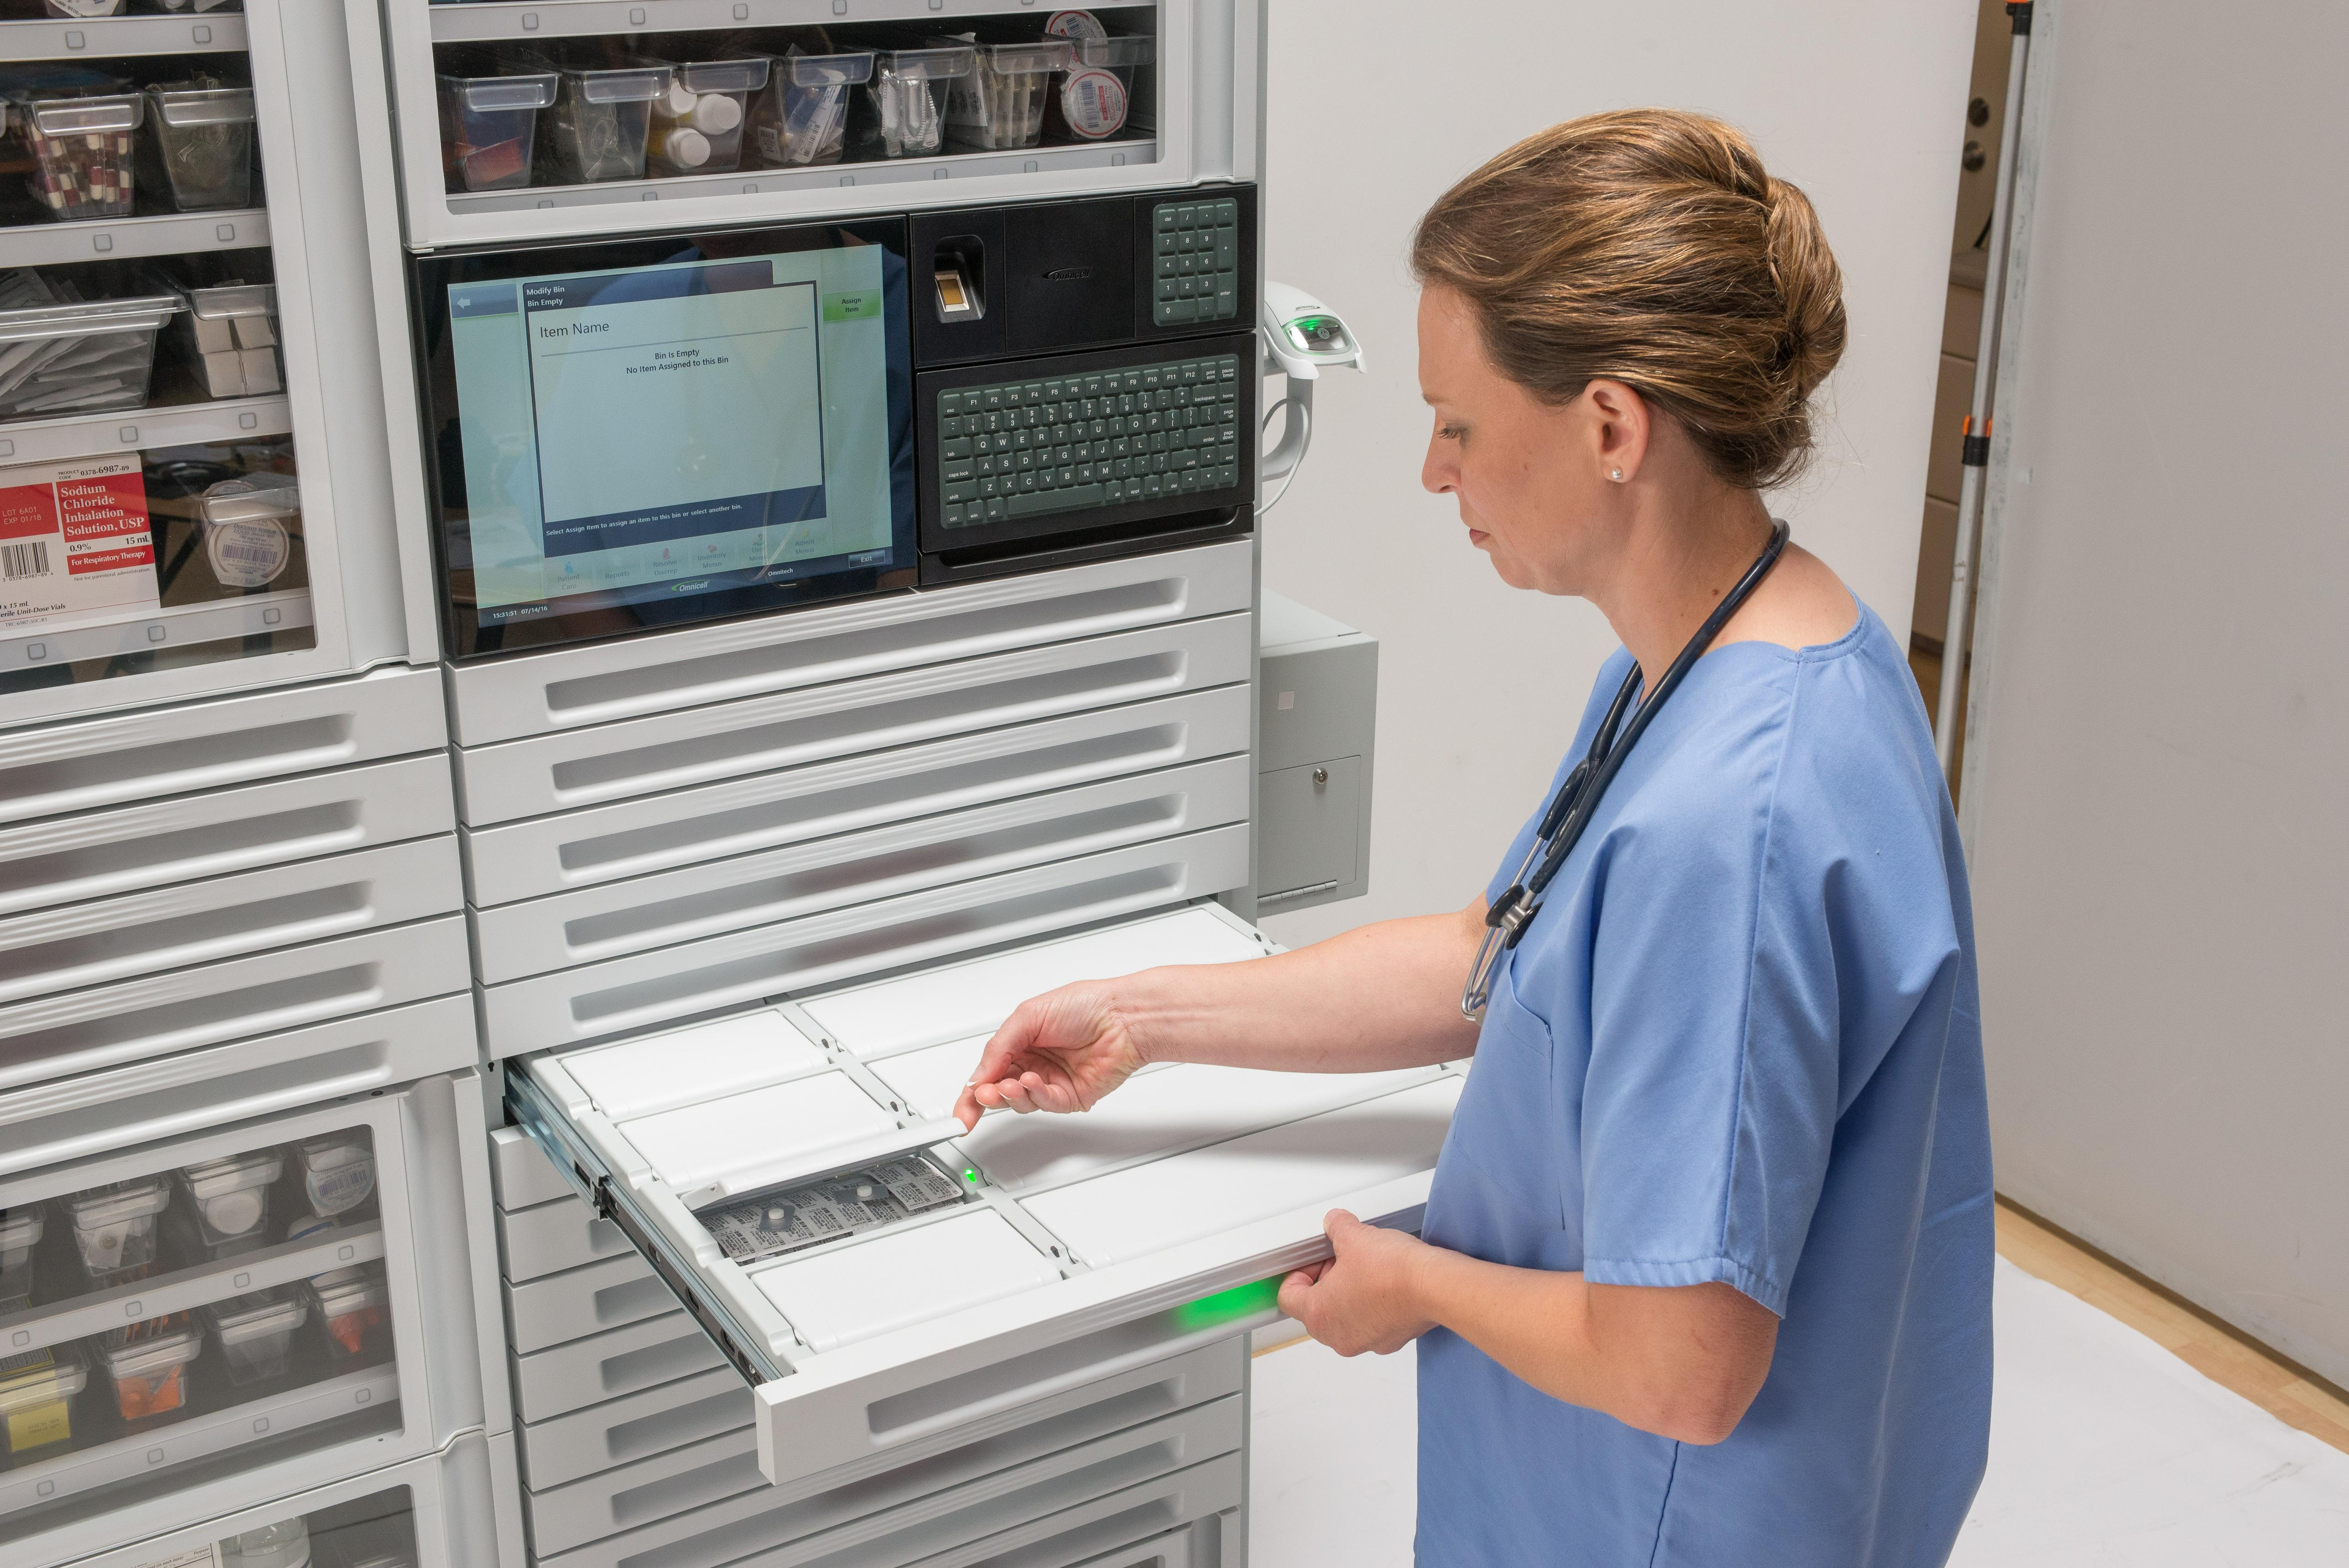
\includegraphics[width=0.445\textwidth,height=3.2cm]{figs/sad.jpeg}
\hspace{0.02\textwidth}
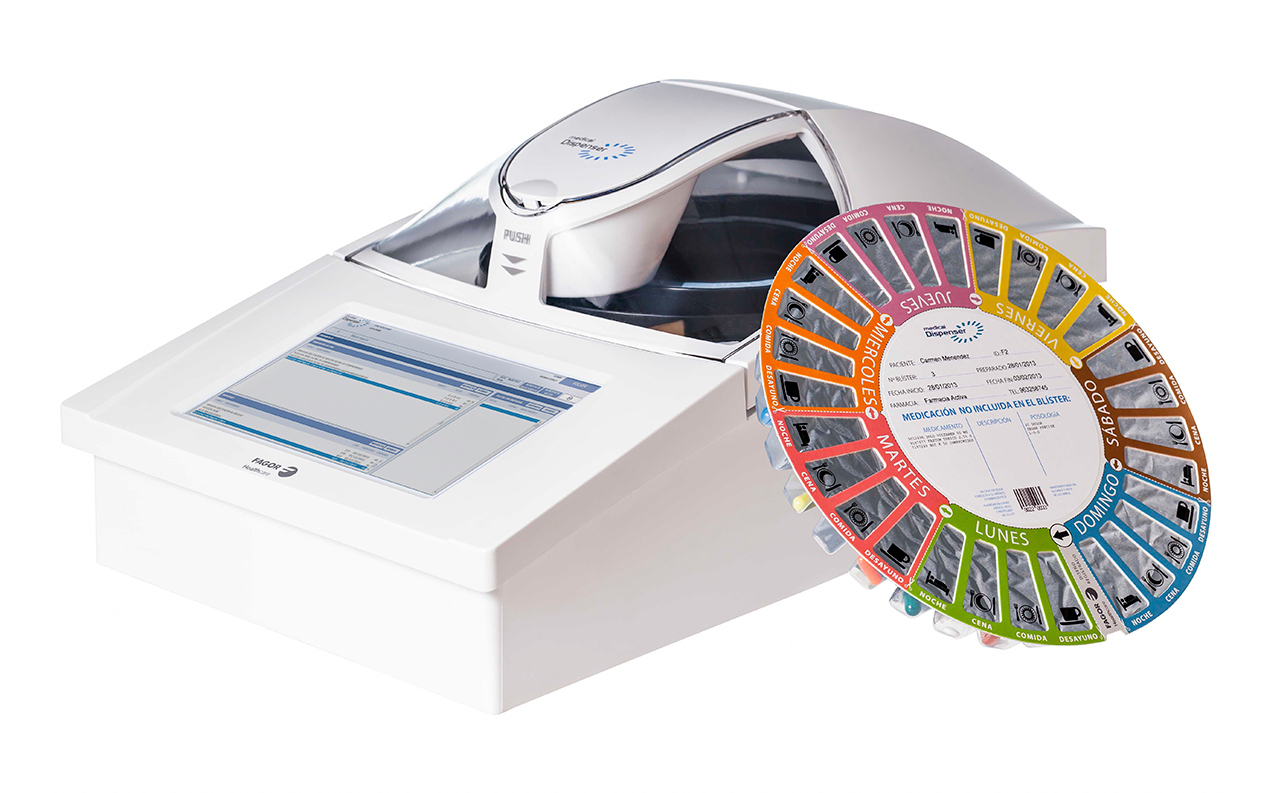
\includegraphics[width=0.445\textwidth,height=3.2cm]{figs/spd.jpg}

\end{figure}

\note[item]{
\item Calidad de vida
\item Envejecimiento + crónicos
\item Atención personalizada
\item $\rightarrow$ Problema medicación
}

\end{frame}

%==================================================
\section*{}
\begin{frame}{}
  \centering \Huge
  \emph{Objetivos}
\note[item]{Uno de los problemas donde estas tecnologías pueden aportar un mayor beneficio es la correcta administración de la medicación.}
\end{frame}

\section{Objetivos}
\subsection{Descripción del problema}
\begin{frame}{Descripción del problema}

\begin{figure}
\centering
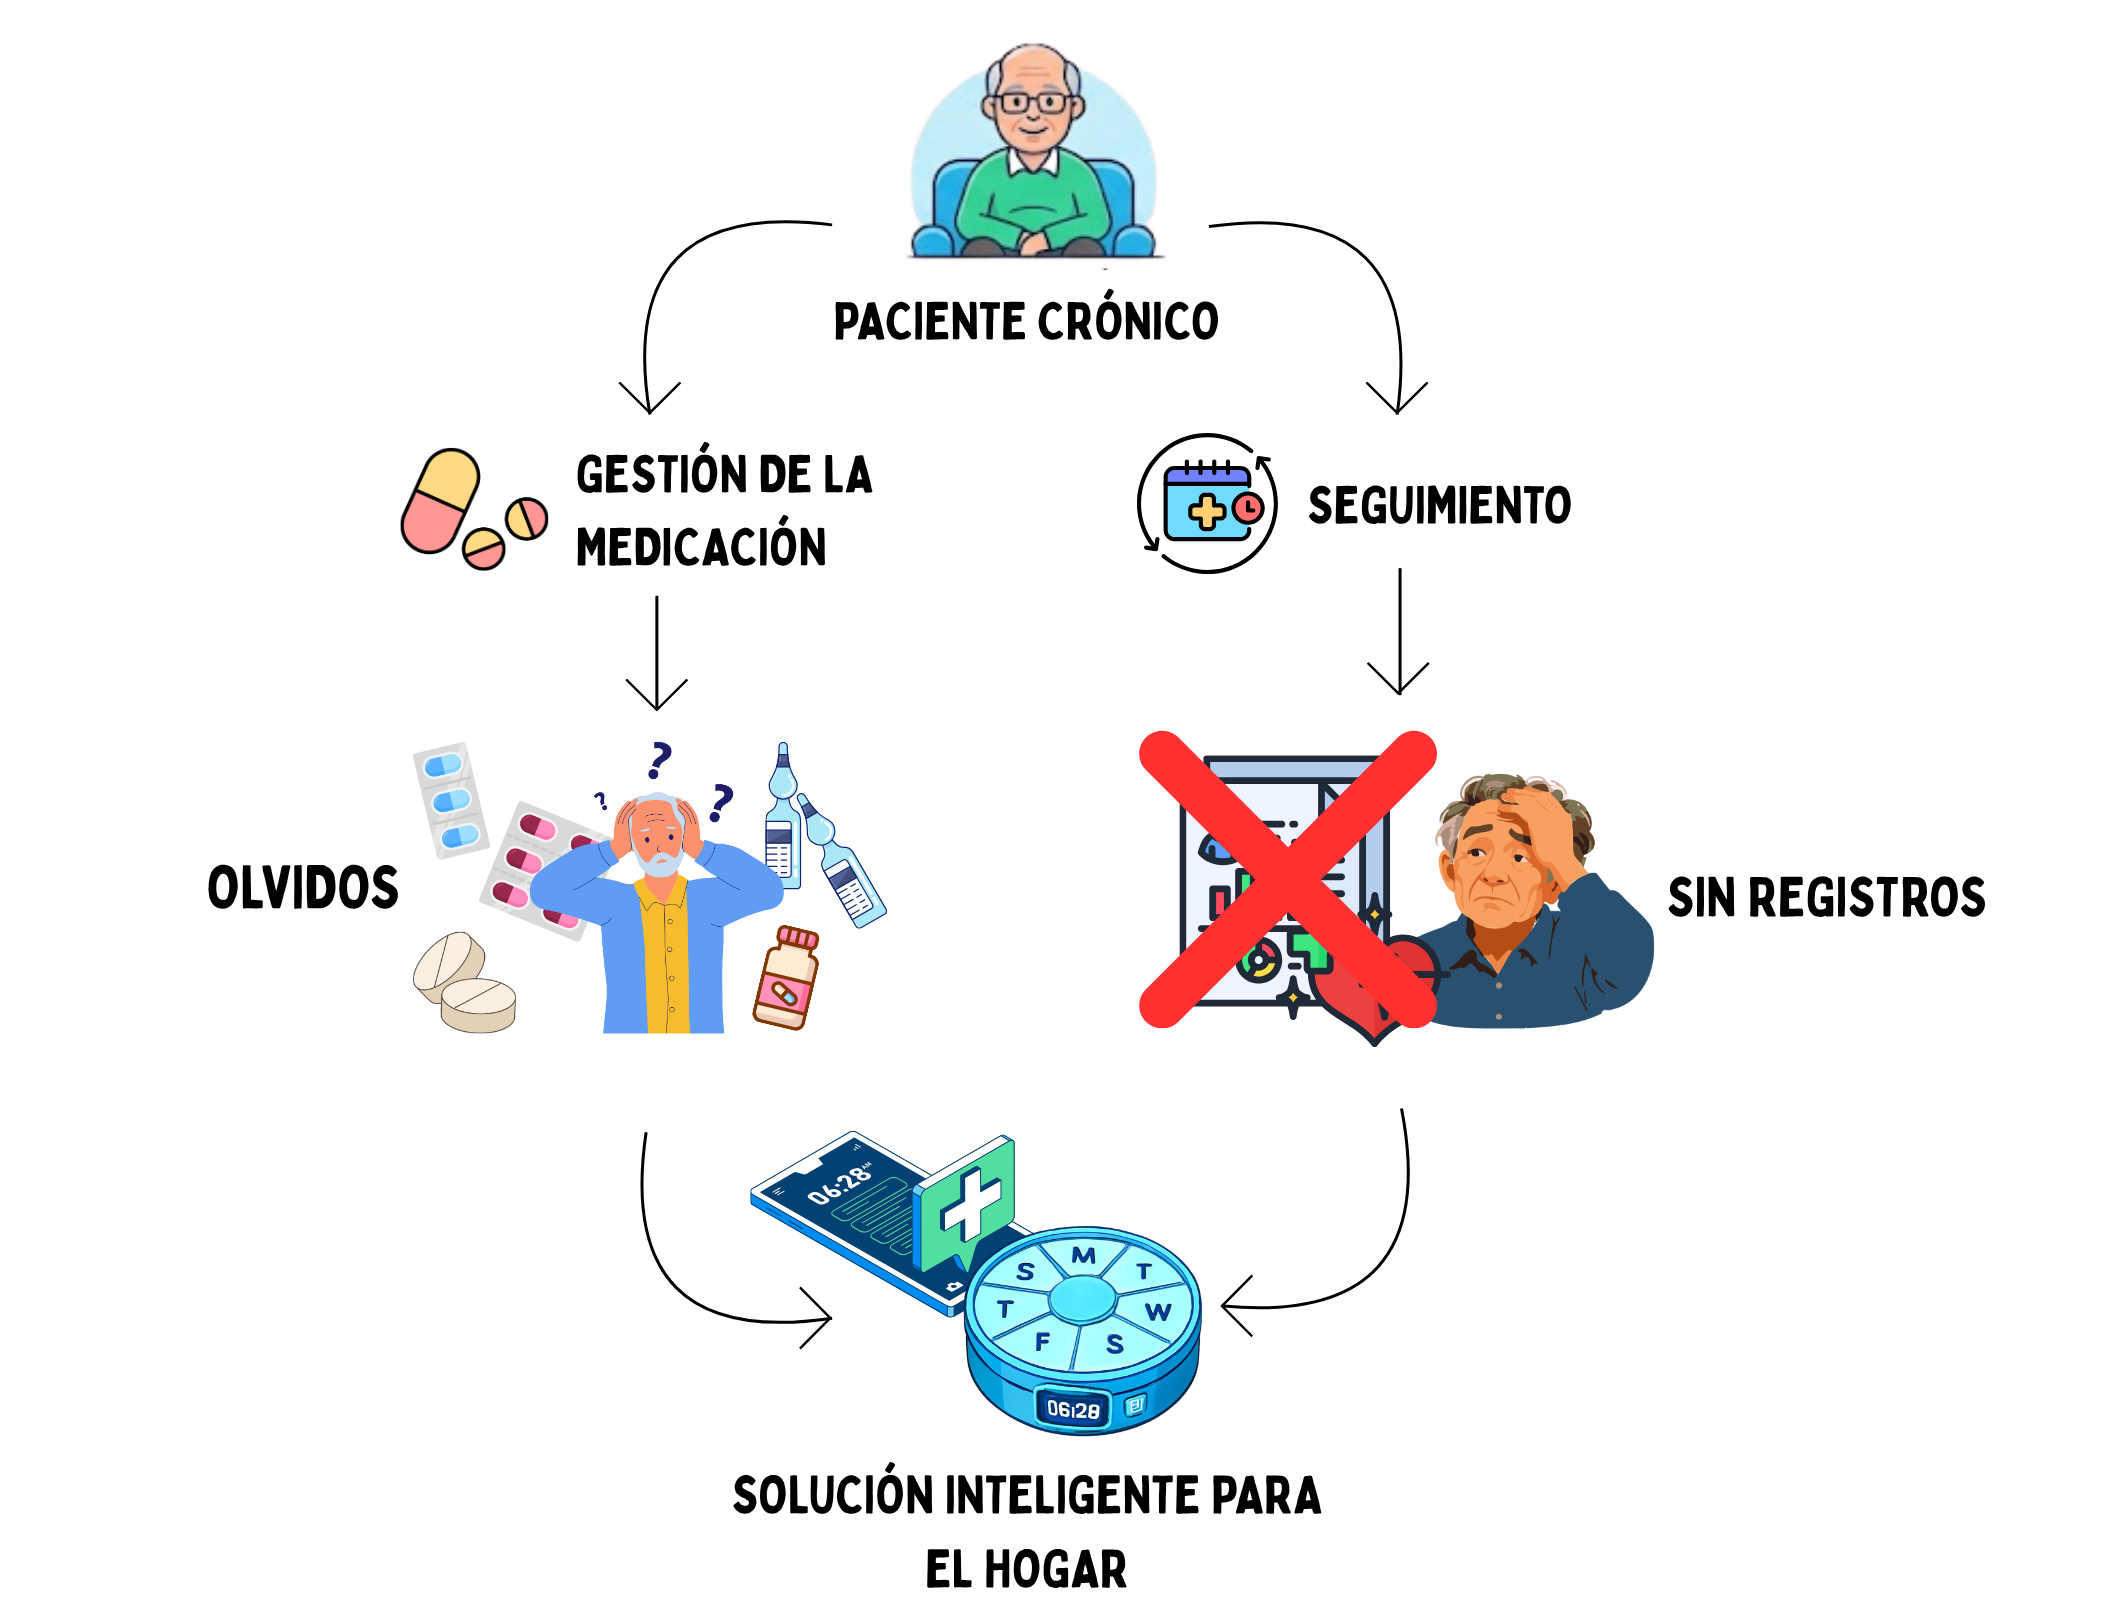
\includegraphics[width=0.8\textwidth]{figs/esquema_problema.png}
\end{figure}

\note[item]{
\item Polimedicación
\item Olvidos / errores
\item Consecuencias salud
\item Dispensadores comerciales
\item Coste elevado
\item MyMeds
\item $\rightarrow$ Objetivos
}
\end{frame}

\subsection{Objetivos}
\begin{frame}
\frametitle{Objetivos}

\begin{block}{Objetivos}
\begin{itemize}
\item Diseñar la \alert{arquitectura general} del sistema.
\item Desarrollar el \alert{diseño mecánico} del pastillero.
\item Integrar el \alert{microcontrolador} y la lógica de control.
\item Implementar una \alert{interfaz táctil} intuitiva.
\item Incorporar un \alert{sensor biomédico}.
\item Desarrollar una \alert{aplicación Android}.
\item Implementar la comunicación \alert{WiFi}.
\item Realizar la \alert{validación experimental}.
\end{itemize}
\end{block}

\note[item]{
\item Objetivo general
\item Dispensación automática
\item Monitorización biomédica
\item Arquitectura
\item Hardware + software
\item App Android
\item Validación
\item $\rightarrow$ Requisitos
}

\end{frame}

\subsection{Requisitos}
\begin{frame}
\frametitle{Requisitos}

\begin{block}{Requisitos}
\begin{itemize}
\item Uso de \alert{ESP32-2432S028}.
\item Desarrollo en \alert{C++} y \alert{Kotlin}.
\item Comunicación mediante \alert{WiFi}.
\item Funcionamiento en \alert{tiempo real}.
\item Fabricación mediante \alert{impresión 3D (PLA)}.
\item Coste inferior a \alert{50\,€}.
\item \alert{Almacenamiento} de medicación y medidas.
\item Avisos \alert{visuales y acústicos}.
\end{itemize}
\end{block}

\note[item]{
\item Bajo coste
\item Impresión 3D
\item ESP32
\item WiFi
\item Avisos
\item Persistencia
\item Interfaz sencilla
\item $\rightarrow$ Metodología
}

\end{frame}

\subsection{Metodología}
\begin{frame}
\frametitle{Metodología}

\begin{figure}
\centering
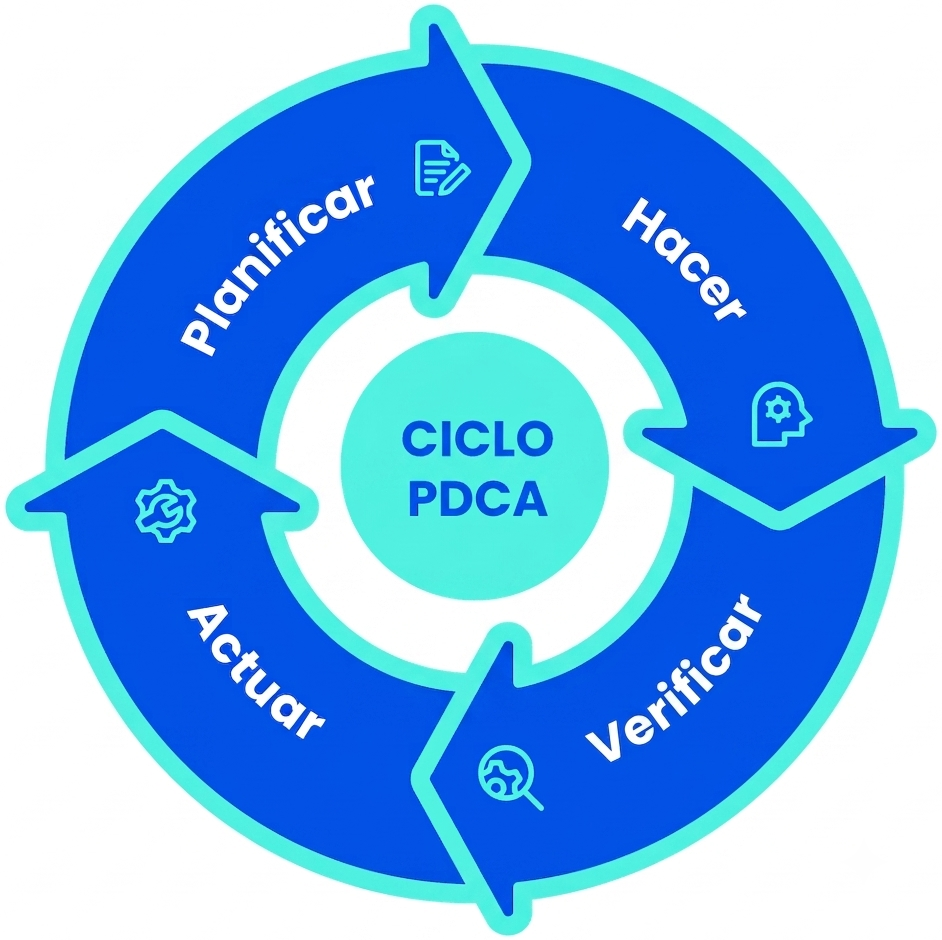
\includegraphics[width=0.36\textwidth]{figs/pdca.png}
\end{figure}

\begin{block}{Metodología de desarrollo}
\begin{itemize}
\item Desarrollo \alert{iterativo} basado en el ciclo \alert{PDCA}.
\item Integración progresiva de los módulos \alert{hardware} y \alert{software}.
\item \alert{Pruebas parciales} tras cada etapa de desarrollo.
\item \alert{Reuniones semanales} con el tutor para revisar el progreso.
\end{itemize}
\end{block}

\note[item]{
\item Ciclo PDCA
\item Planificar
\item Implementar
\item Verificar
\item Mejorar
\item Desarrollo iterativo
\item $\rightarrow$ Plataforma
}

\end{frame}


%==================================================
\section*{}
\begin{frame}{}
  \centering \Huge
  \emph{Plataforma de desarrollo}
\end{frame}

\section{Plataforma de desarrollo}
\subsection{Hardware}
\begin{frame}
\frametitle{Hardware}

\begin{center}

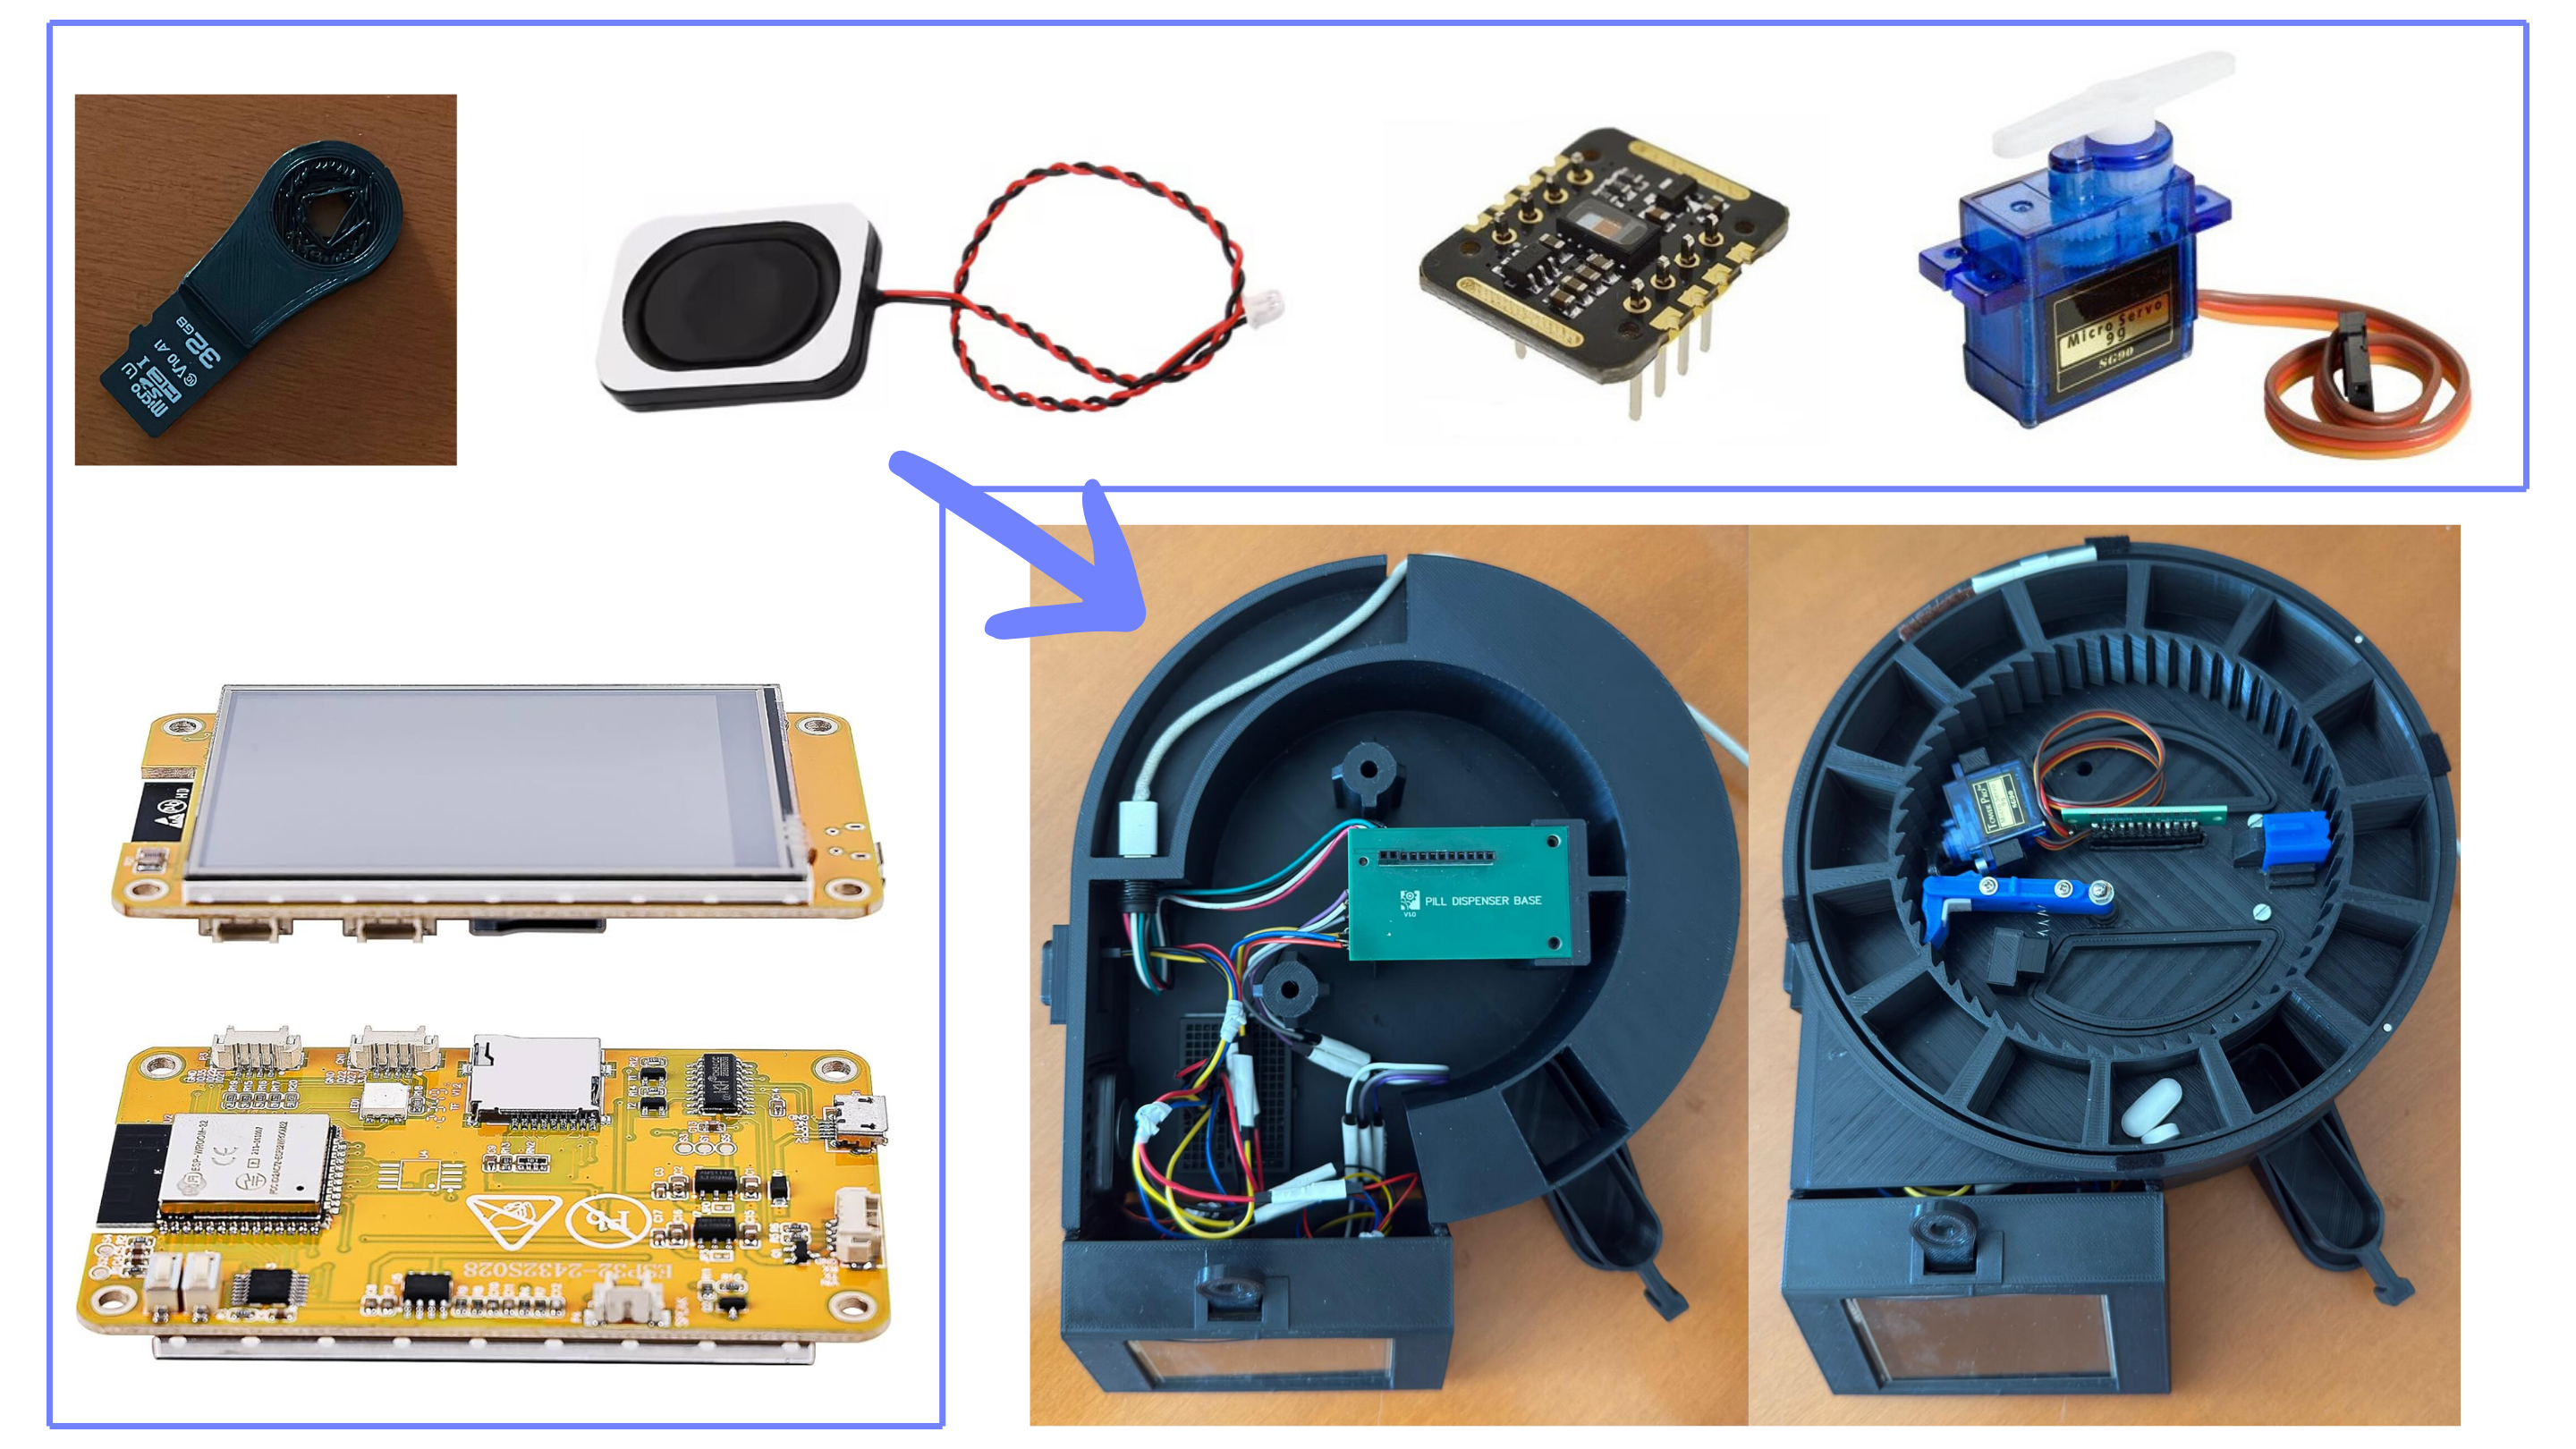
\includegraphics[width=\textwidth]{figs/hard.png}

\end{center}

\note[item]{
\item ESP32-2432S028
\item MCU + TFT + WiFi
\item PCB personalizada
\item PCA9685
\item MAX30102 + I2C
\item Protoboard
\item Trinquete + muelle
\item Carcasa 3D
\item $\rightarrow$ Software
}

\end{frame}

\subsection{Software}
\begin{frame}
\frametitle{Software}

\begin{center}

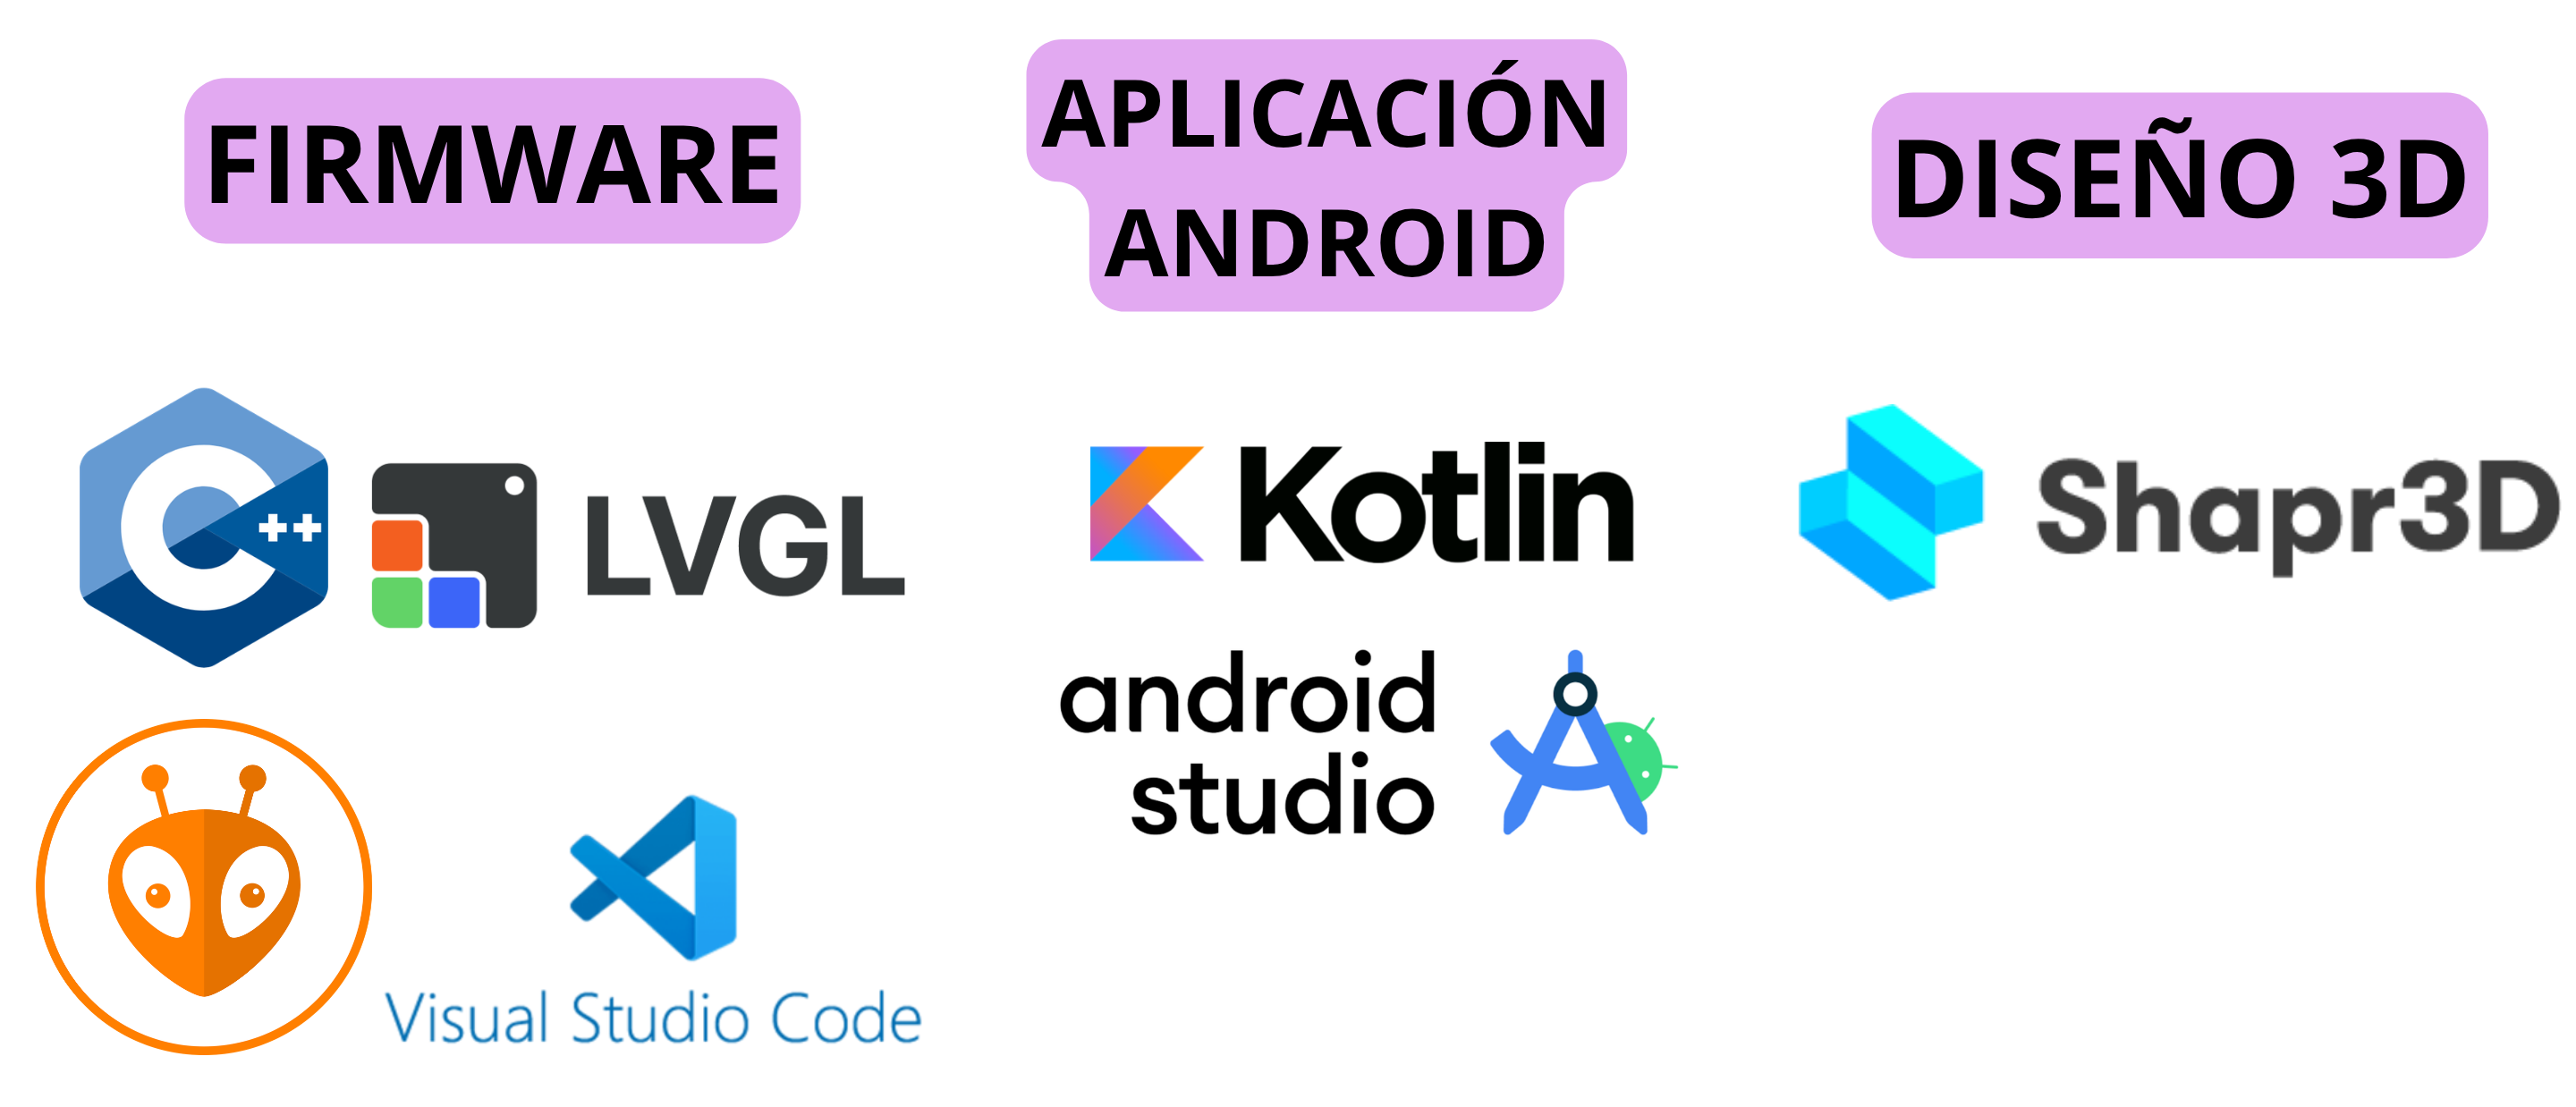
\includegraphics[width=\textwidth]{figs/software.png}

\end{center}

\note[item]{
\item 3 herramientas
\item PlatformIO (firmware)
\item Android Studio (app)
\item Sharp3D (CAD)
\item Cada una → módulo
\item $\rightarrow$ Arquitectura
}

\end{frame}

%==================================================
\section*{}
\begin{frame}{}
  \centering \Huge
  \emph{Diseño del sistema}
\end{frame}

\section{Diseño del sistema}
\subsection{Arquitectura general}

\begin{frame}
\frametitle{Arquitectura general del sistema}

\begin{center}
    
\includegraphics[width=\textwidth]{figs/arquitectura_sistema.jpg}
\end{center}

\note[item]{
\item Firmware = núcleo
\item Inicialización
\item Configuración persistente
\item Comunicación App
\item UI + planificación
\item Dispensación
\item Pulsómetro
\item WiFi + almacenamiento
\item Sistema embebido
\item $\rightarrow$ App
}

\end{frame}

\subsection{Aplicación móvil}
\begin{frame}
\frametitle{Aplicación móvil}

\begin{center}
    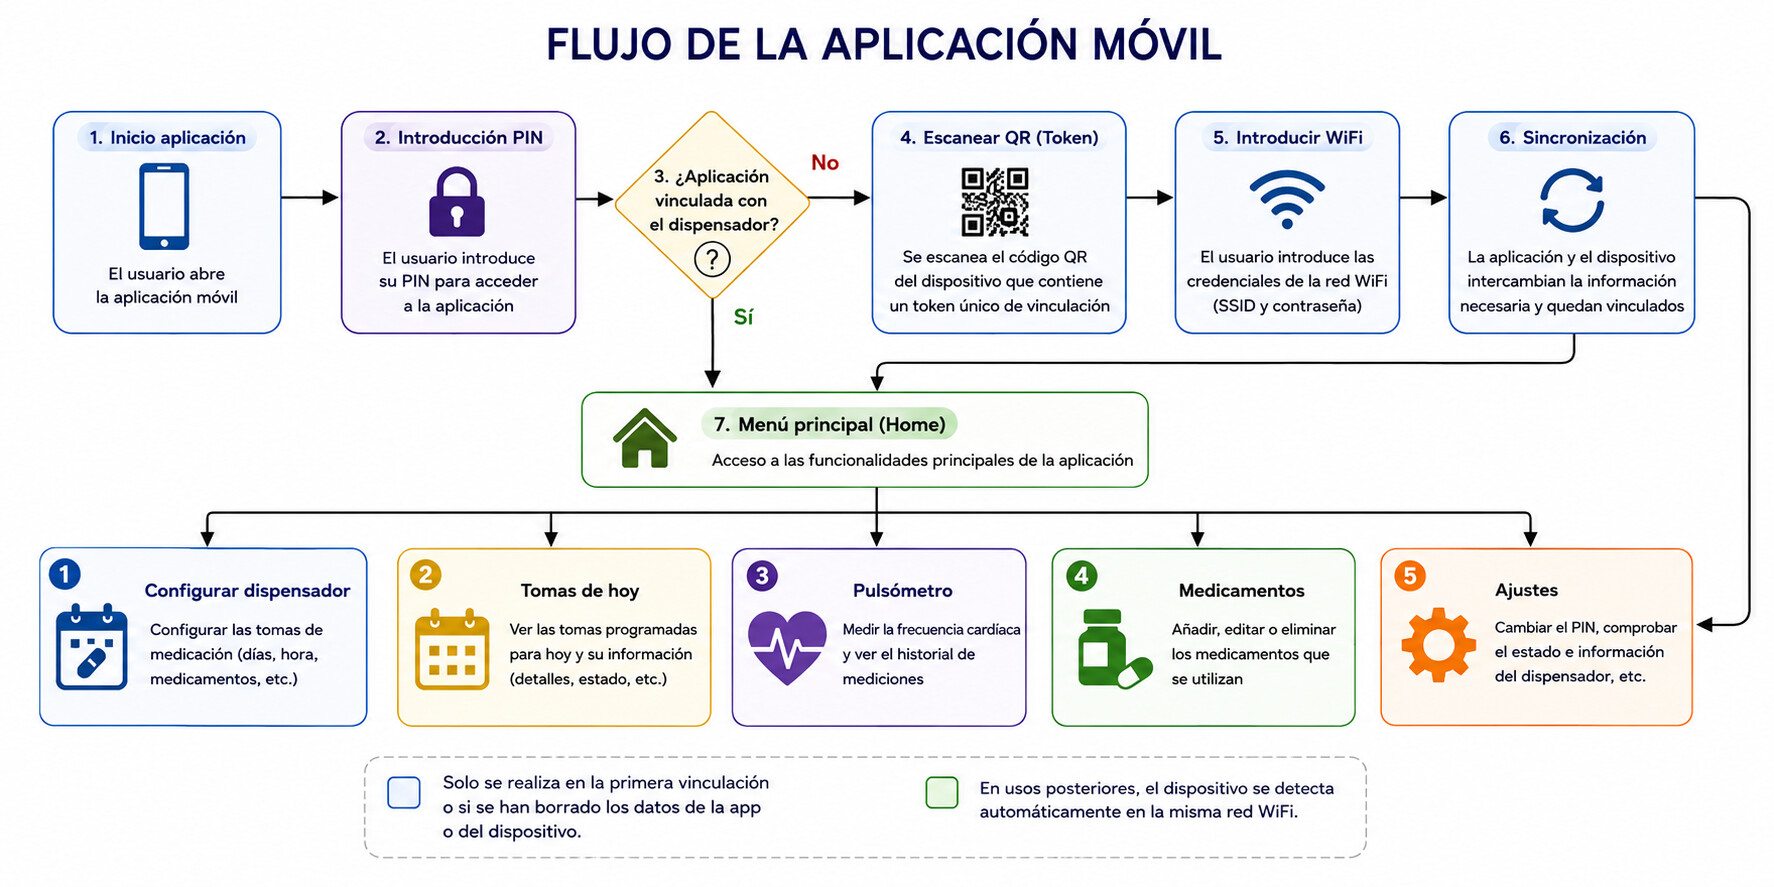
\includegraphics[width=0.97\textwidth]{figs/flujo_app.jpg}
    \caption{[Elaboración propia con IA]}
\end{center}

\note[item]{
\item Punto interacción
\item QR
\item Vinculación segura
\item Menú principal
\item Medicamentos
\item Tomas
\item Historial
\item Sincronización WiFi
\item Centro gestión
\item Experimentos
}

\end{frame}

%==================================================
\section*{}
\begin{frame}{}
  \centering \Huge
  \emph{Validación experimental}
\end{frame}

\section{Validación experimental}
\subsection{Sistema de dispensación}

\begin{frame}
\frametitle{Validación del sistema de dispensación}

\begin{columns}[c]

\column{0.5\textwidth}
\centering
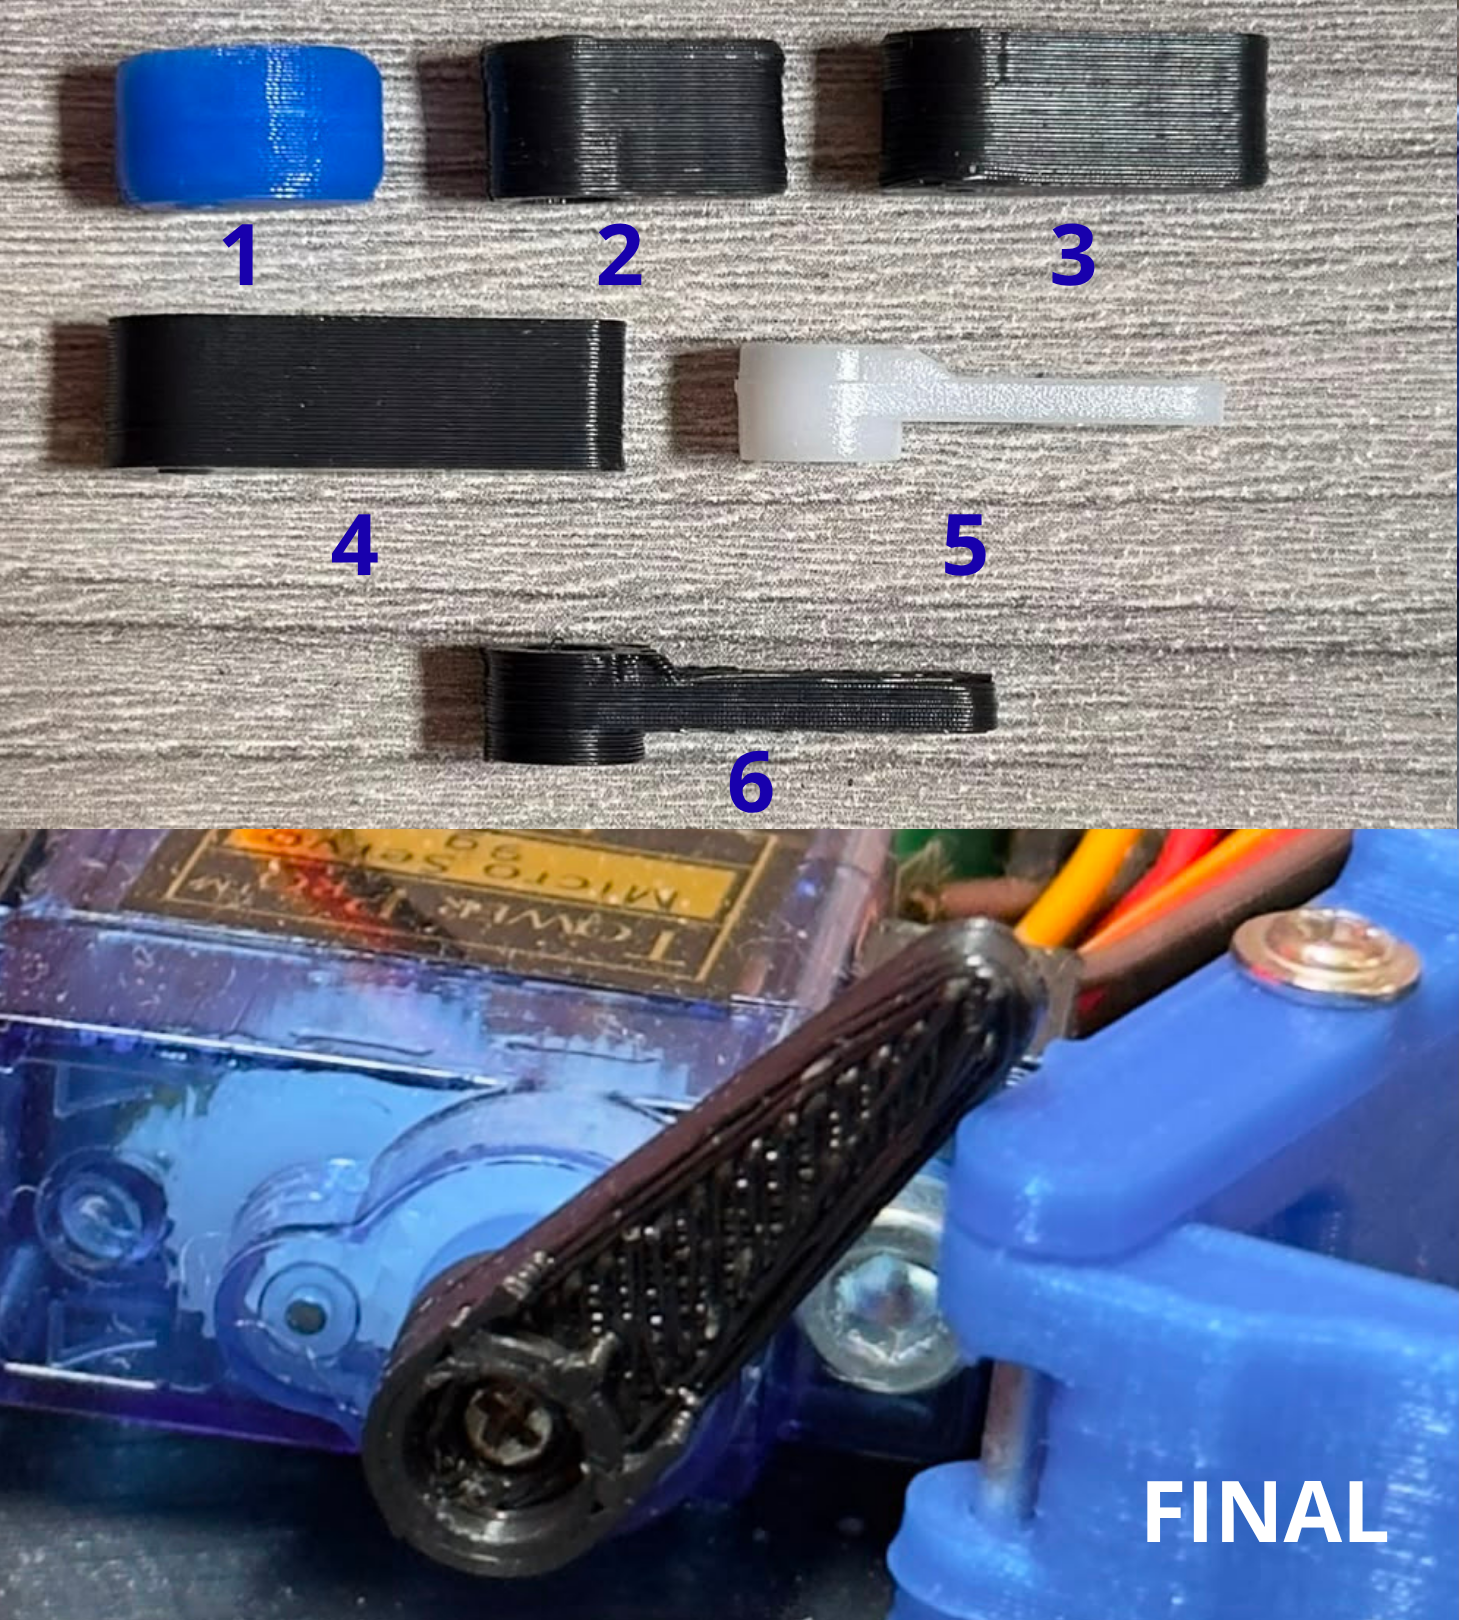
\includegraphics[width=0.85\linewidth]{figs/evolucion_impulsor.png}

{\small\textbf{Evolución del impulsor}}

\column{0.5\textwidth}
\centering
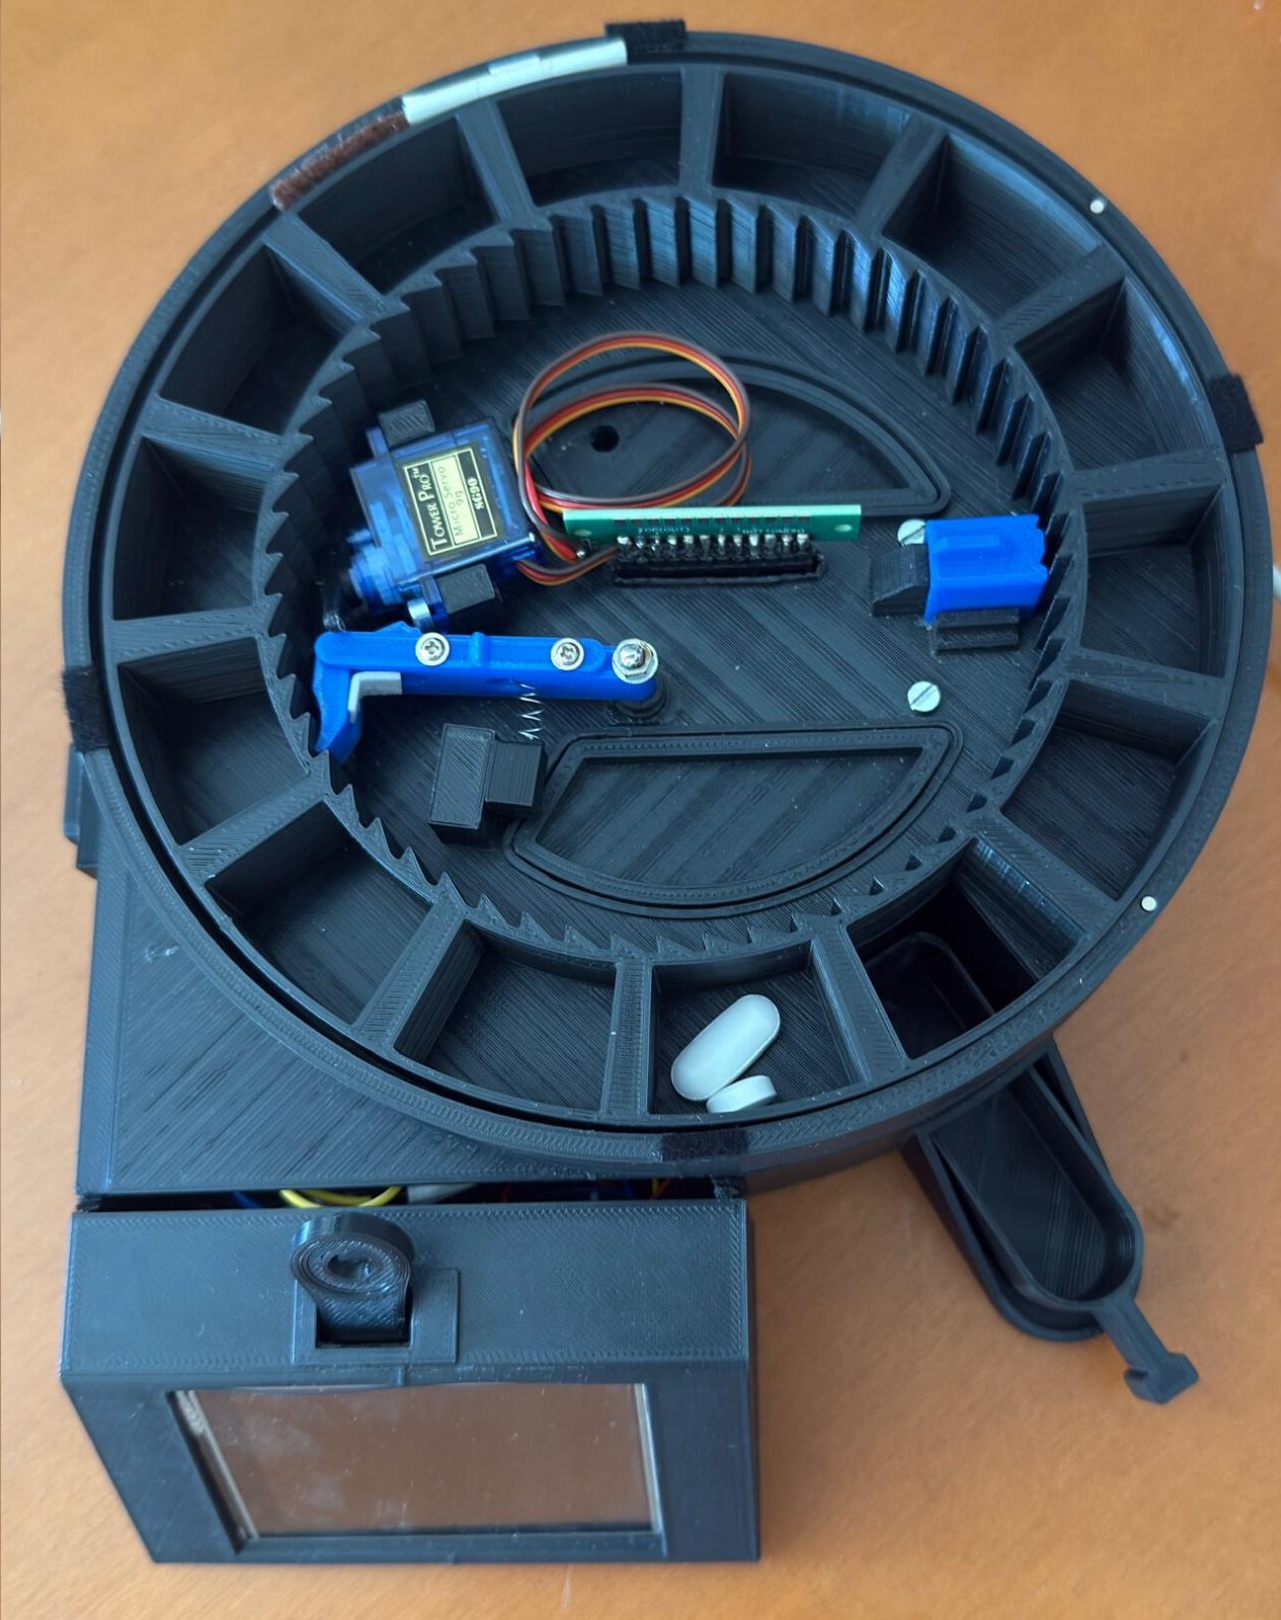
\includegraphics[width=0.85\linewidth]{figs/mecanismo.jpg}

\vspace{0.2cm}

{\small\textbf{Mecanismo definitivo}}

\end{columns}

\vspace{0.4cm}

\note[item]{
\item 4 accionamientos
\item 1 dosis
\item Ajustes mecánicos
\item Impulsor
\item Muelle
\item Alineación
\item Validación App + ESP
\item $\rightarrow$ MAX30102
}

\end{frame}

\subsection{Integración MAX30102}

\begin{frame}
\frametitle{Integración del sensor MAX30102}

\begin{center}
    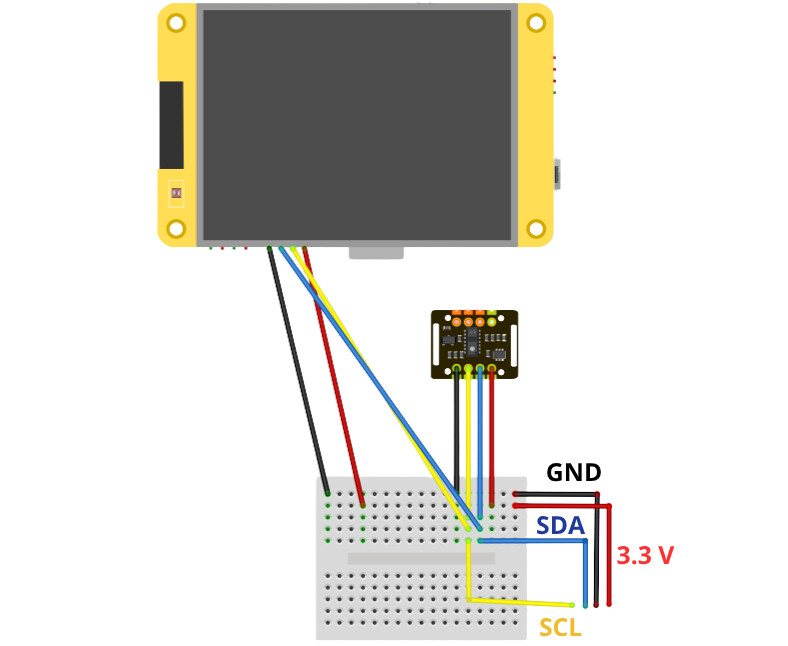
\includegraphics[width=0.7\textwidth]{figs/esquema.jpg}
\end{center}

\note[item]{
\item Fotopletismografía
\item FC + SpO2
\item LEDs
\item Luz reflejada
\item Validación sensor
\item Estabilización
}
\end{frame}

\begin{frame}
\frametitle{Procesamiento de la señal PPG}

\begin{center}
    
\includegraphics[width=0.95\textwidth]{figs/sensor_esquema.jpg}
\end{center}

\note{
El sensor ilumina el dedo mediante LEDs rojo e infrarrojo y el fotodiodo recoge la luz reflejada por el flujo sanguíneo.

A partir de esta señal PPG se detectan los picos correspondientes a cada latido, se calcula el intervalo entre pulsos y se obtiene la frecuencia cardíaca instantánea.

Finalmente, el firmware aplica un promedio y un filtro exponencial para reducir el ruido y mejorar la estabilidad de las medidas antes de mostrarlas al usuario.
}
\end{frame}

\begin{frame}
\frametitle{Resultados experimentales del sensor}

\begin{center}
    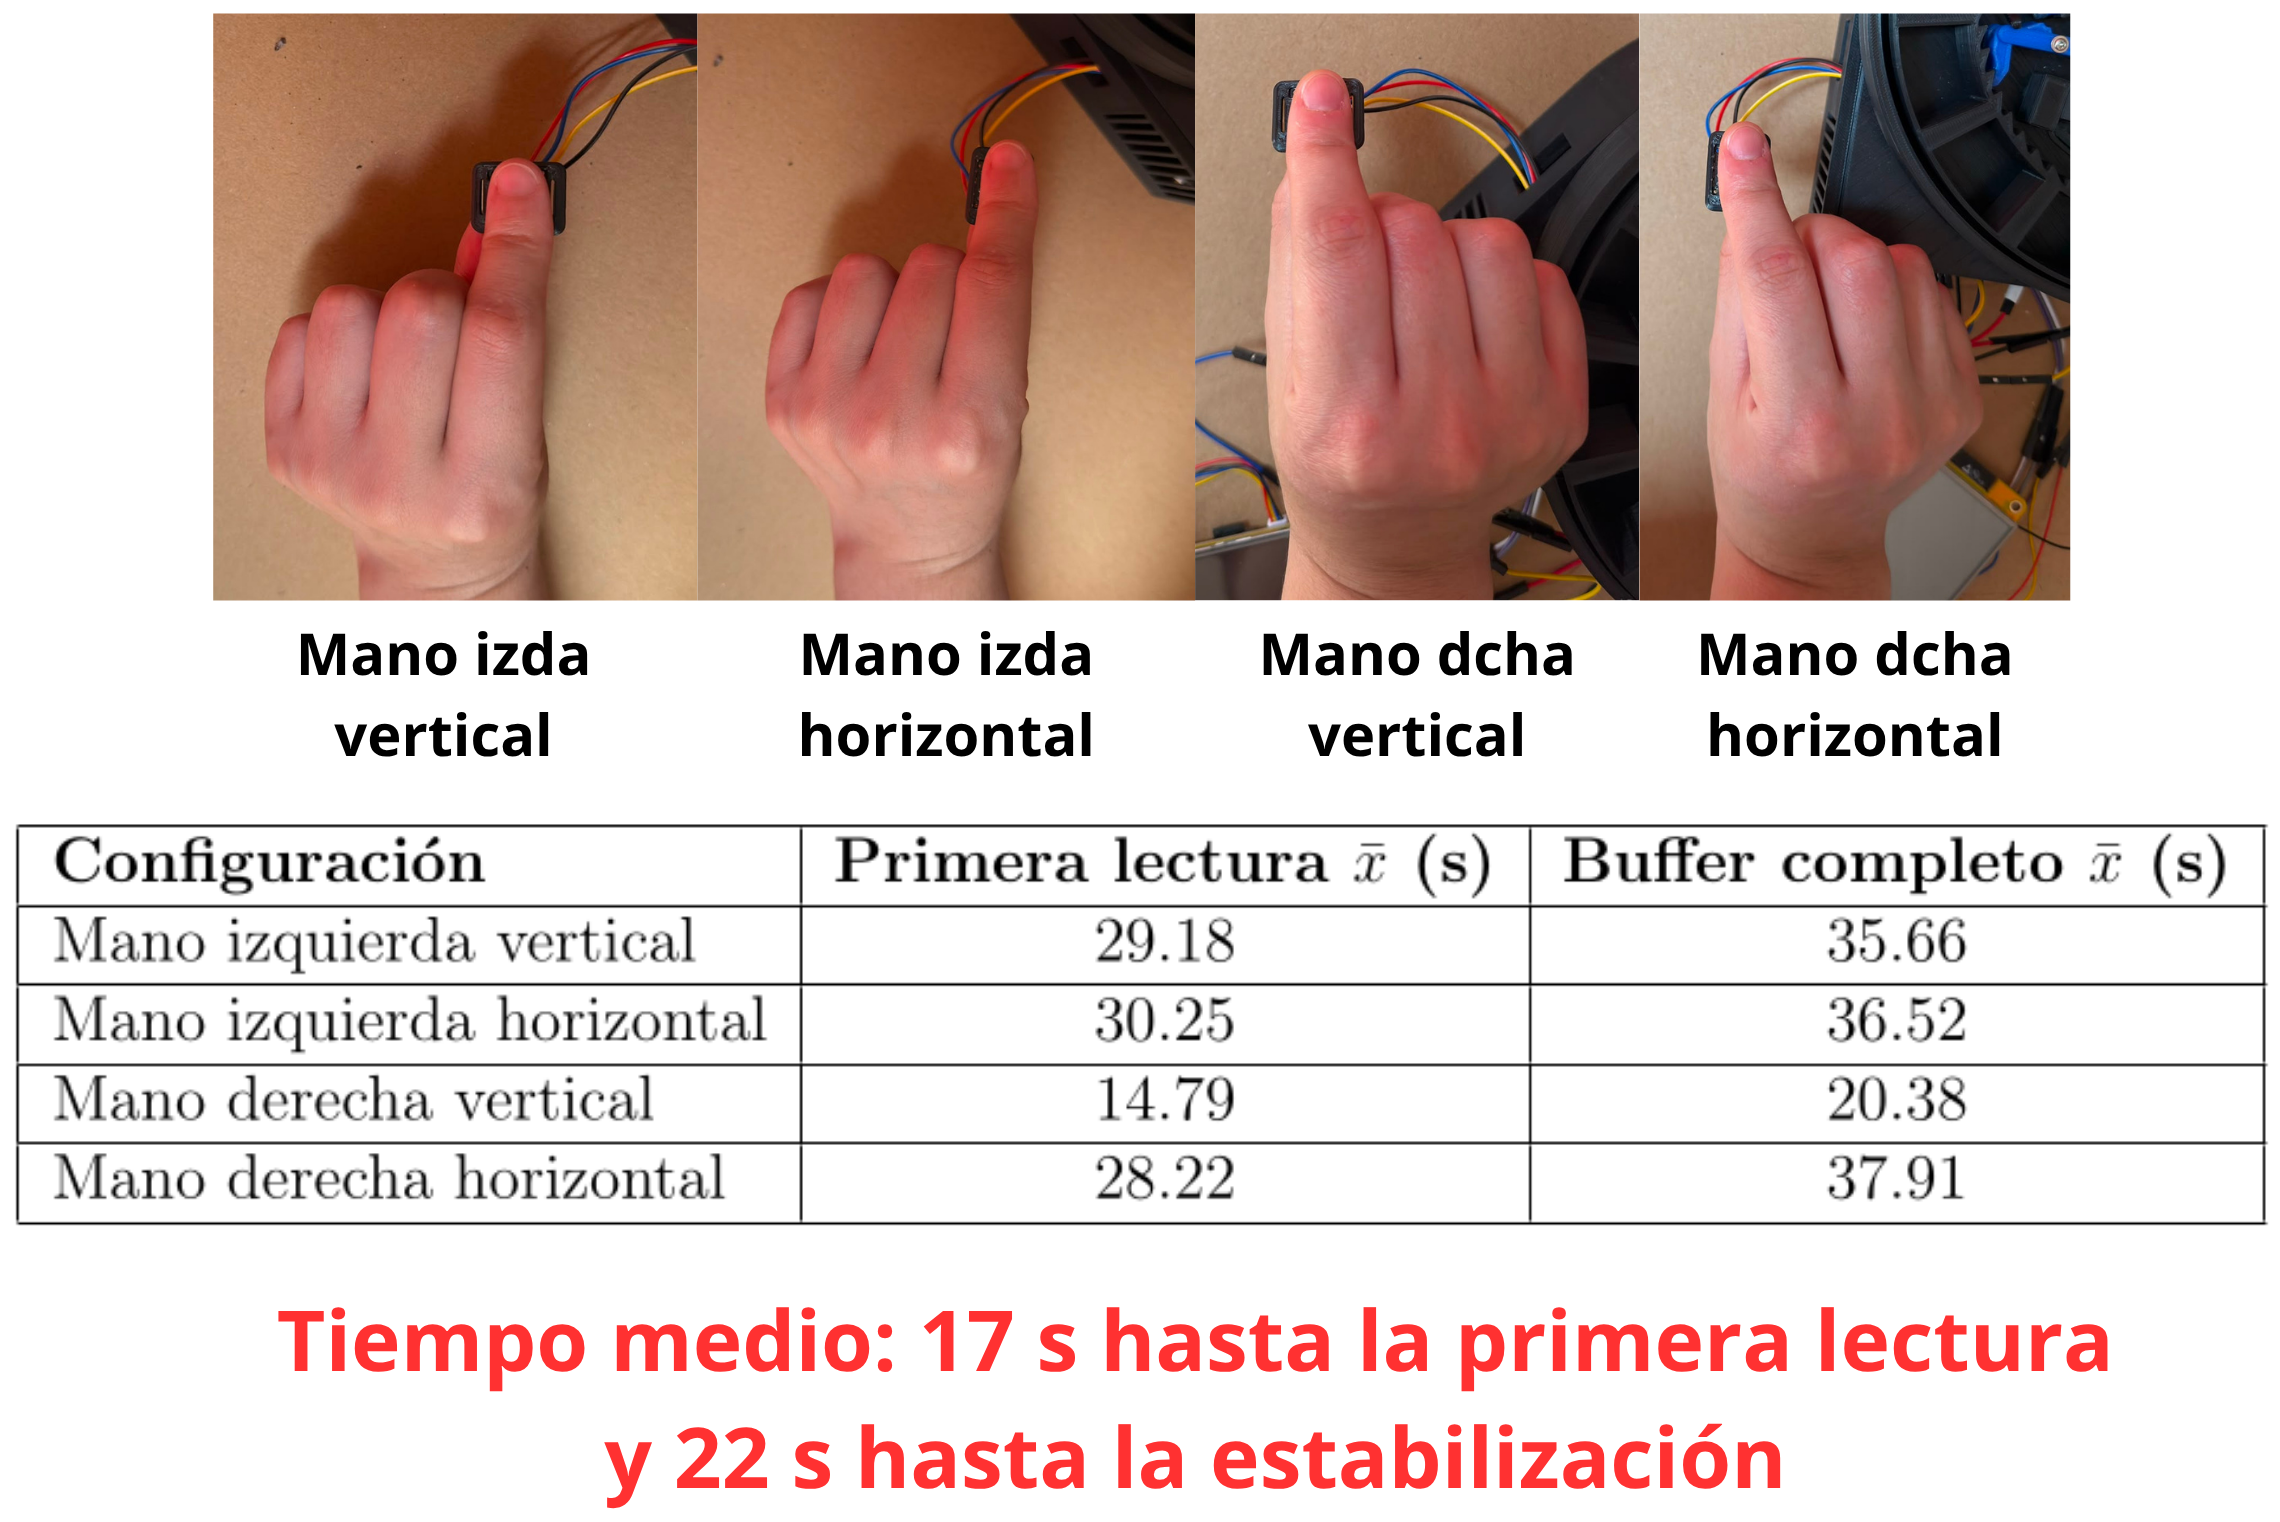
\includegraphics[width=0.95\textwidth]{figs/experimento_sensor.png}
\end{center}

\note[item]{
\item Primera lectura
\item Estabilización
\item 17 s
\item 22 s
\item Sensor óptico
\item $\rightarrow$ Posición
}

\end{frame}

\begin{frame}
\frametitle{Comparación con pulsioxímetro comercial}

\begin{center}
    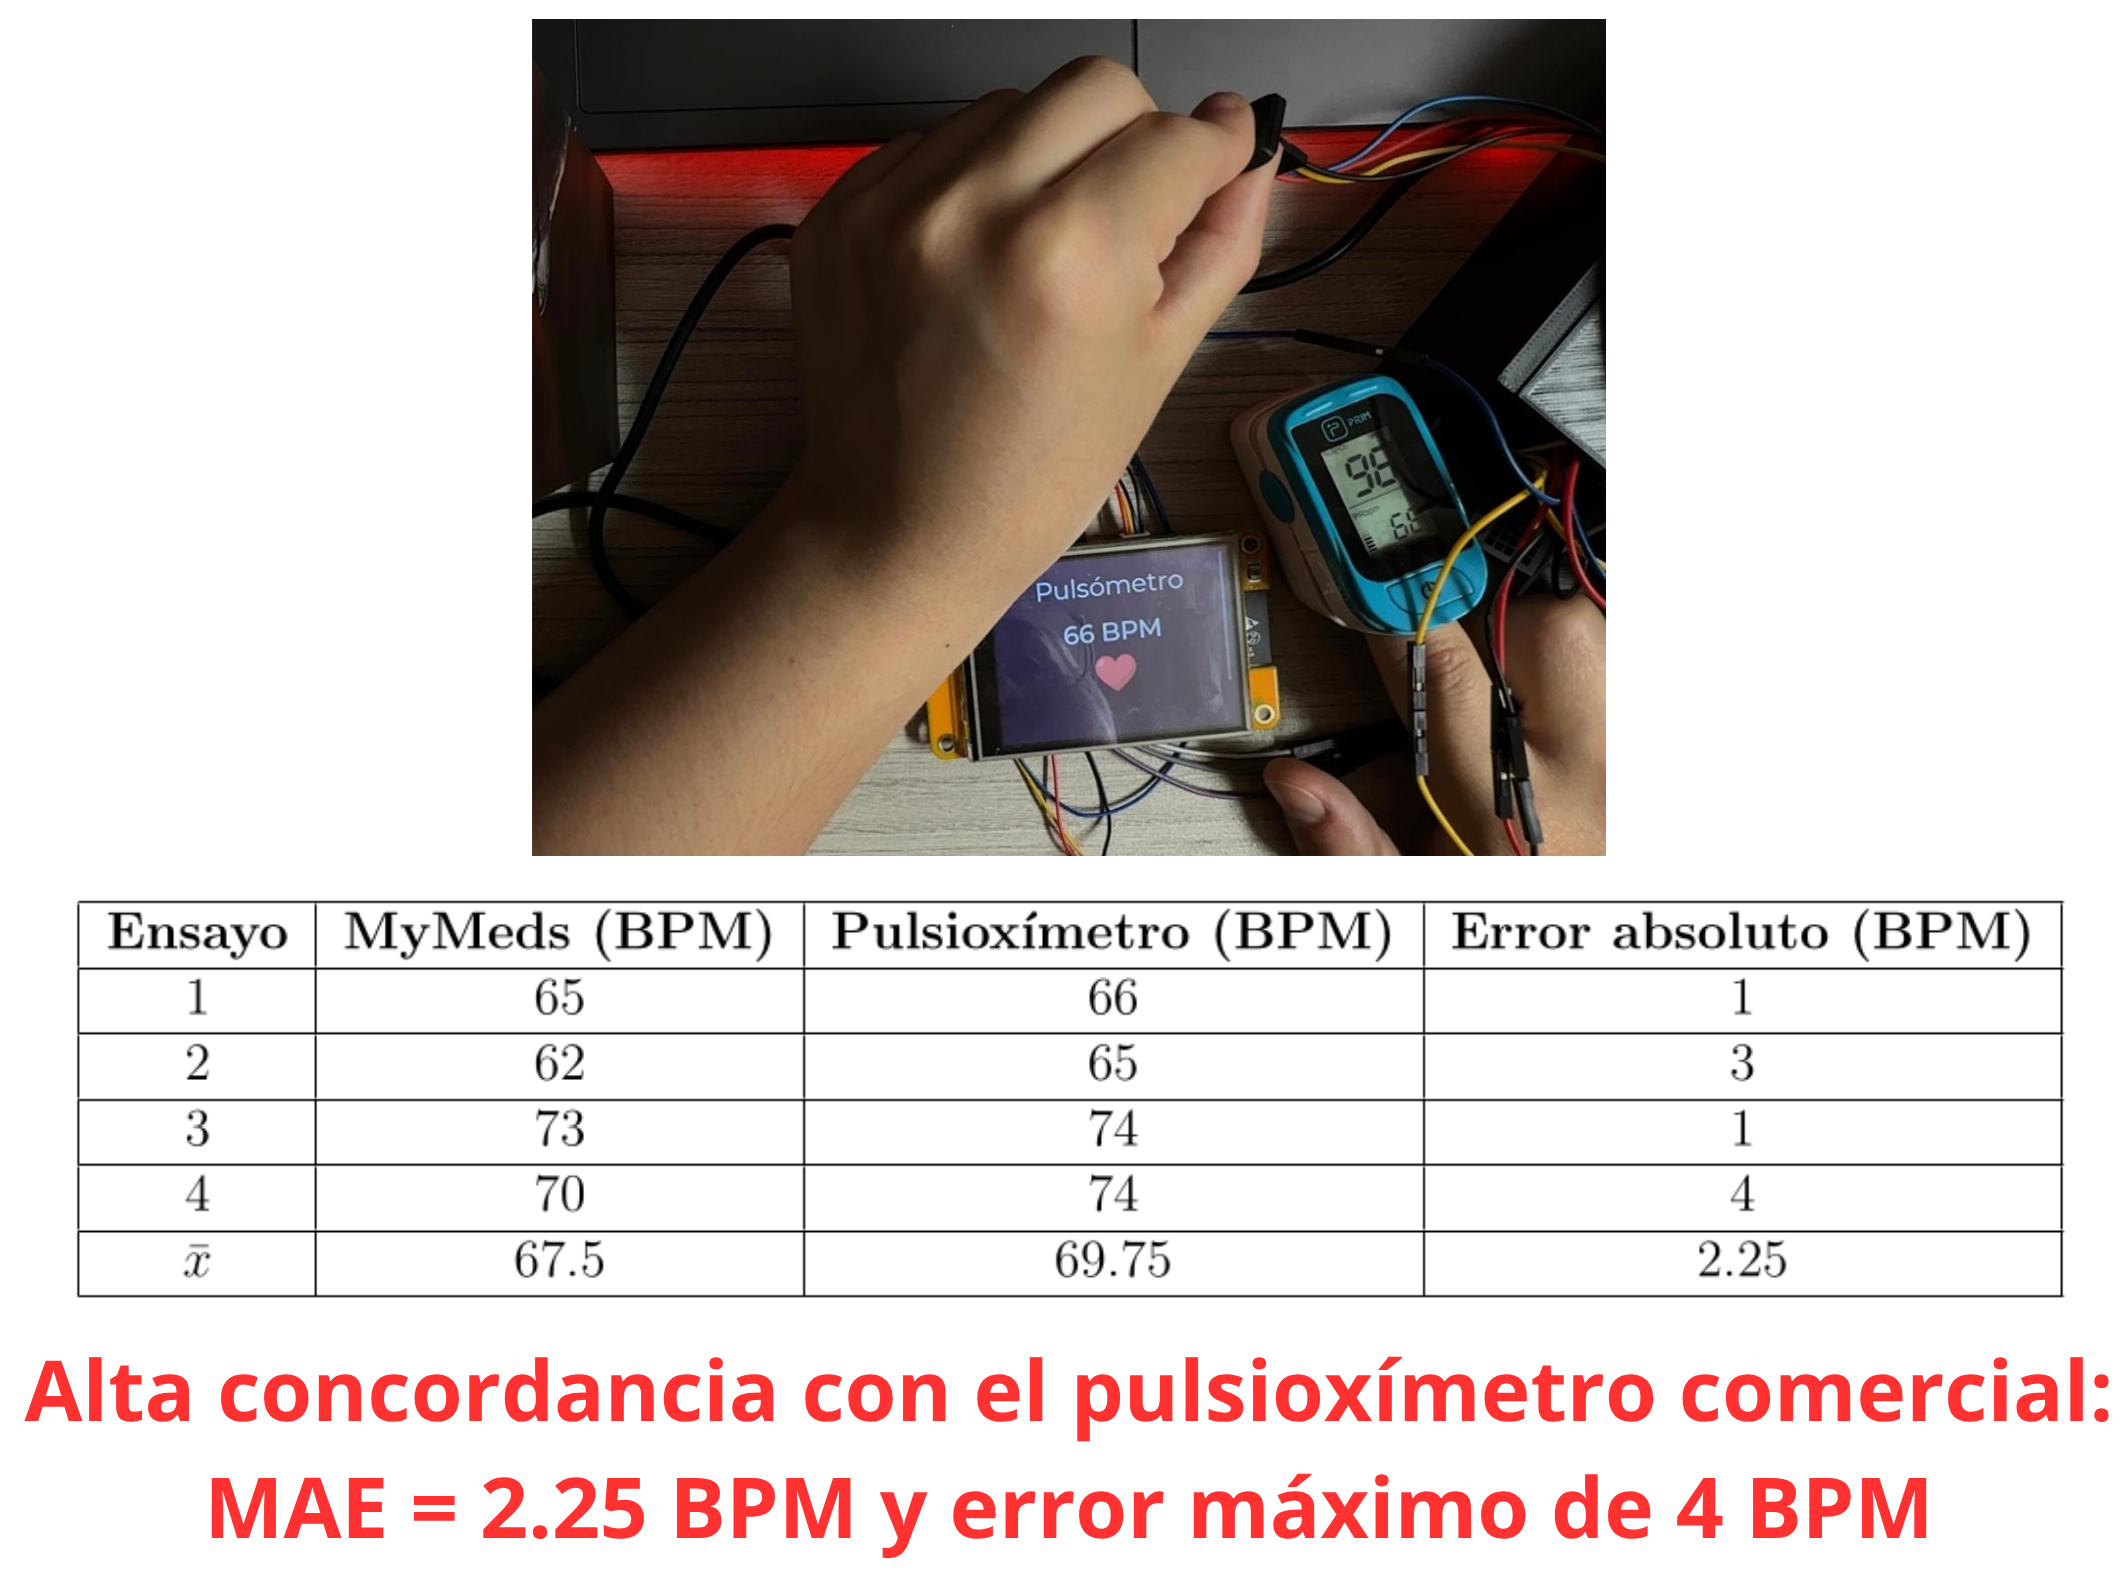
\includegraphics[width=0.85\textwidth]{figs/experimento_comercial.png}
\end{center}

\note[item]{
\item Pulsioxímetro referencia
\item Error medio 2,25 BPM
\item Error máx. 4 BPM
\item Resultados consistentes
\item No dispositivo médico
\item Persistencia
}

\end{frame}

\subsection{Persistencia y almacenamiento}

\begin{frame}
\frametitle{Persistencia de la configuración}

\begin{center}
    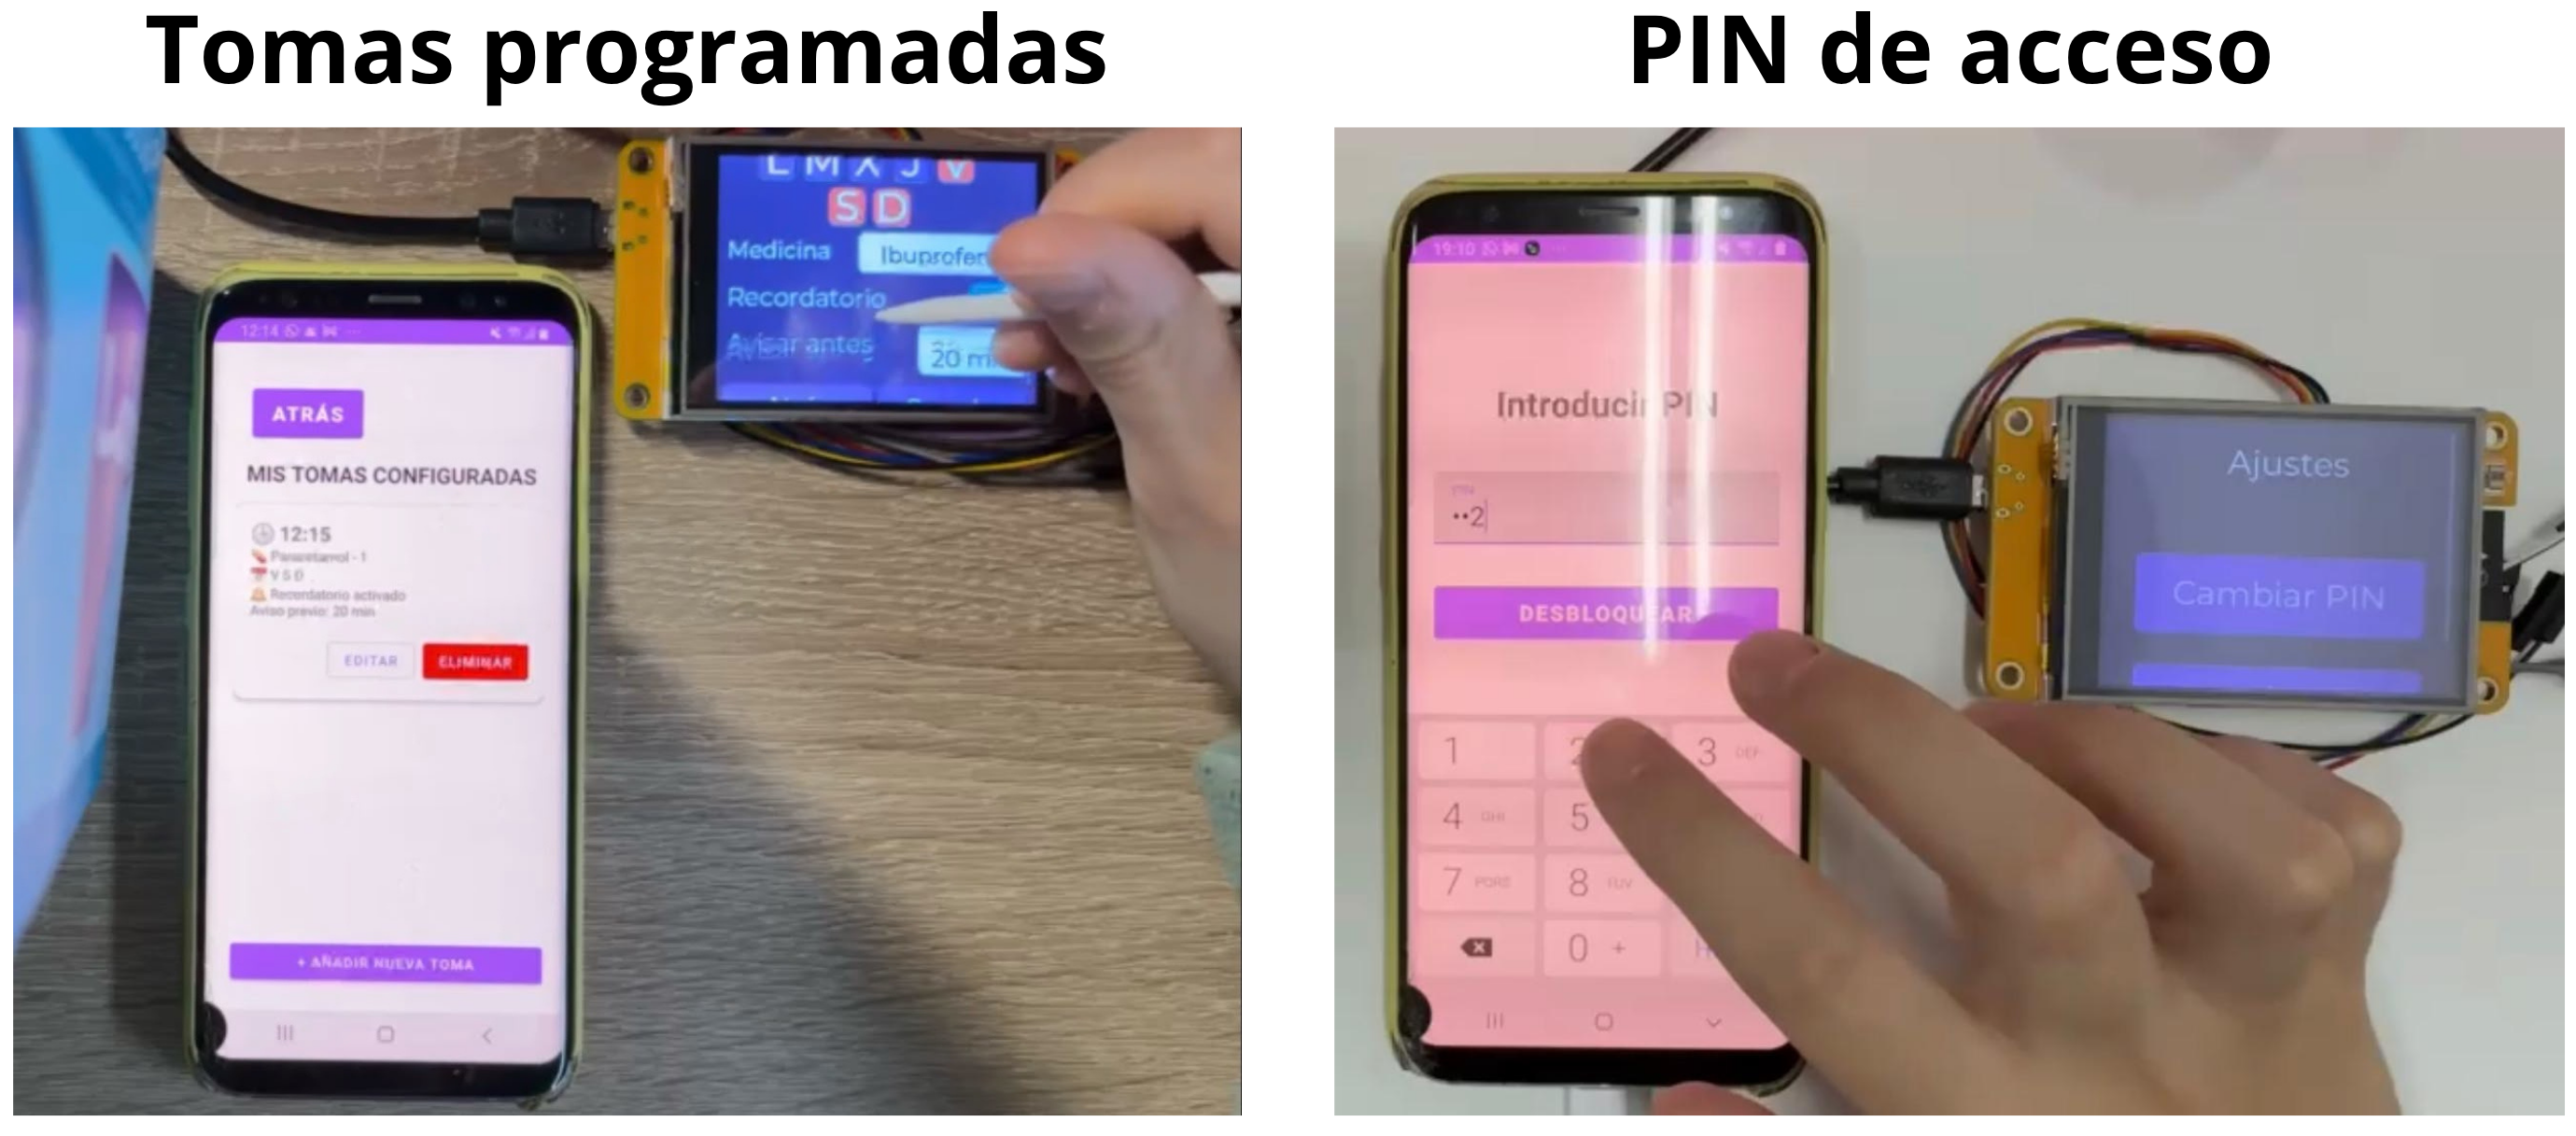
\includegraphics[width=\textwidth]{figs/conservacion.png}
\end{center}

\note[item]{
\item Reinicio ESP32
\item Configuración intacta
\item Medicamentos
\item Tomas
\item Persistencia
\item Historial

}

\end{frame}

\begin{frame}
\frametitle{Historial de medidas}

\begin{center}
    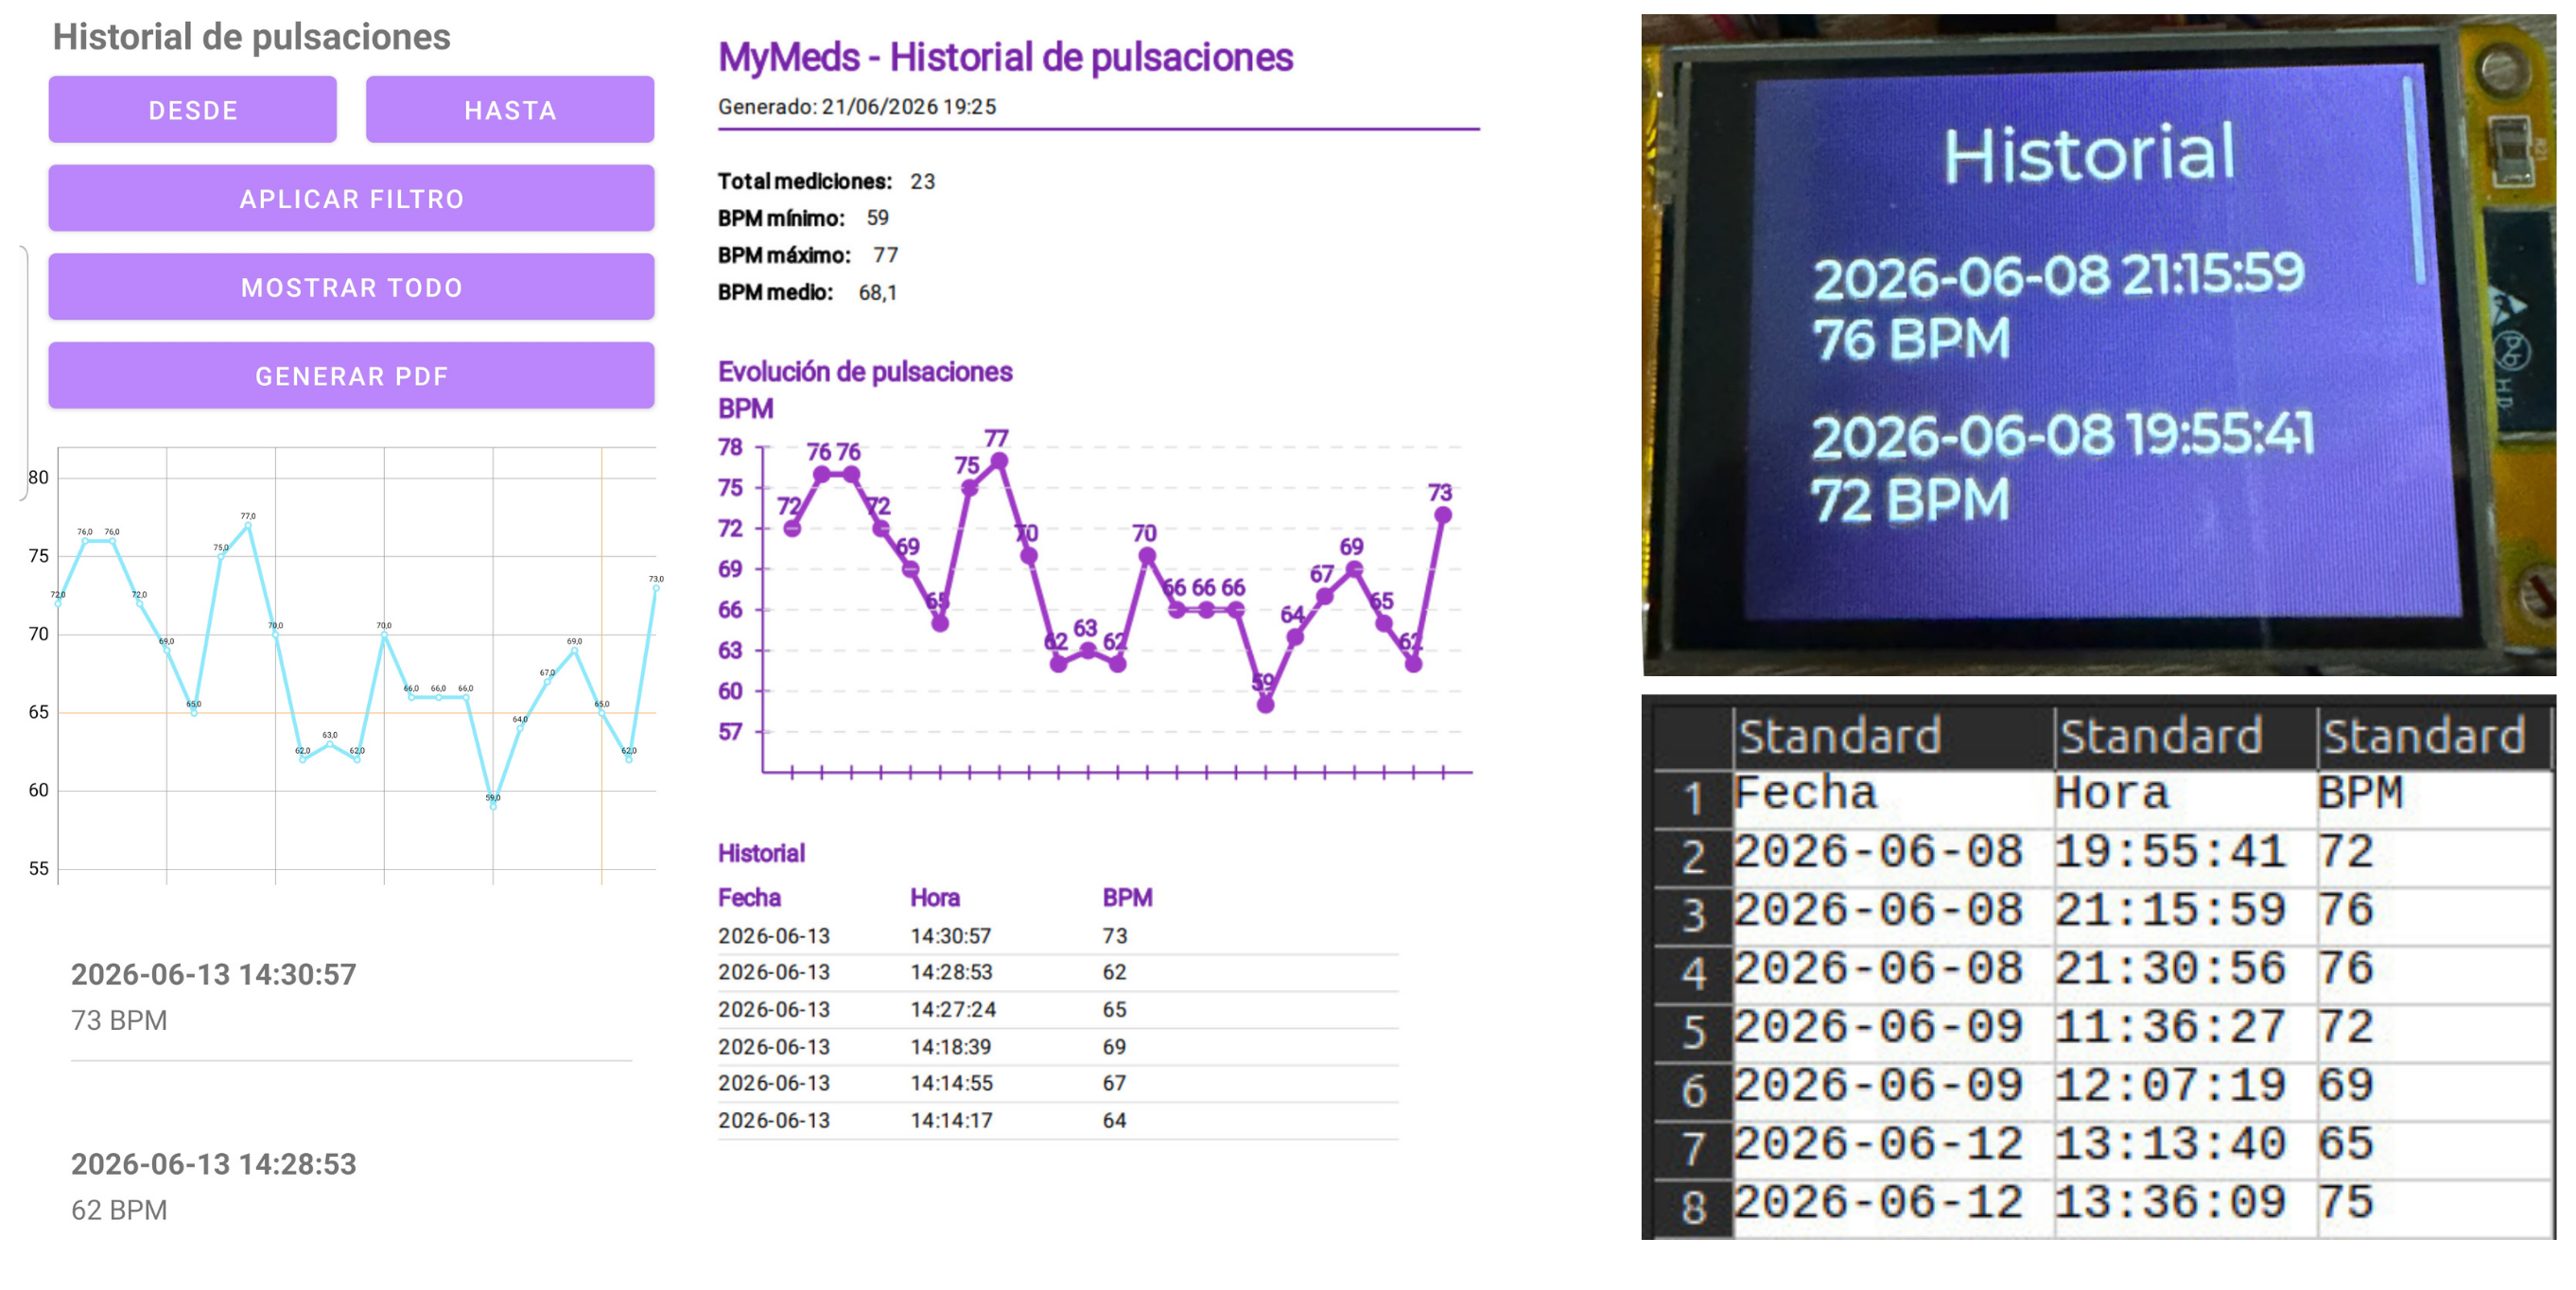
\includegraphics[width=\textwidth]{figs/datos.png}
\end{center}

\note[item]{
\item microSD
\item Fecha + hora
\item Historial App
\item Exportación PDF
\item Sin pérdida datos
\item $\rightarrow$ Seguridad
}

\end{frame}

\subsection{Seguridad}

\begin{frame}
\frametitle{Proceso de autenticación}

\begin{center}
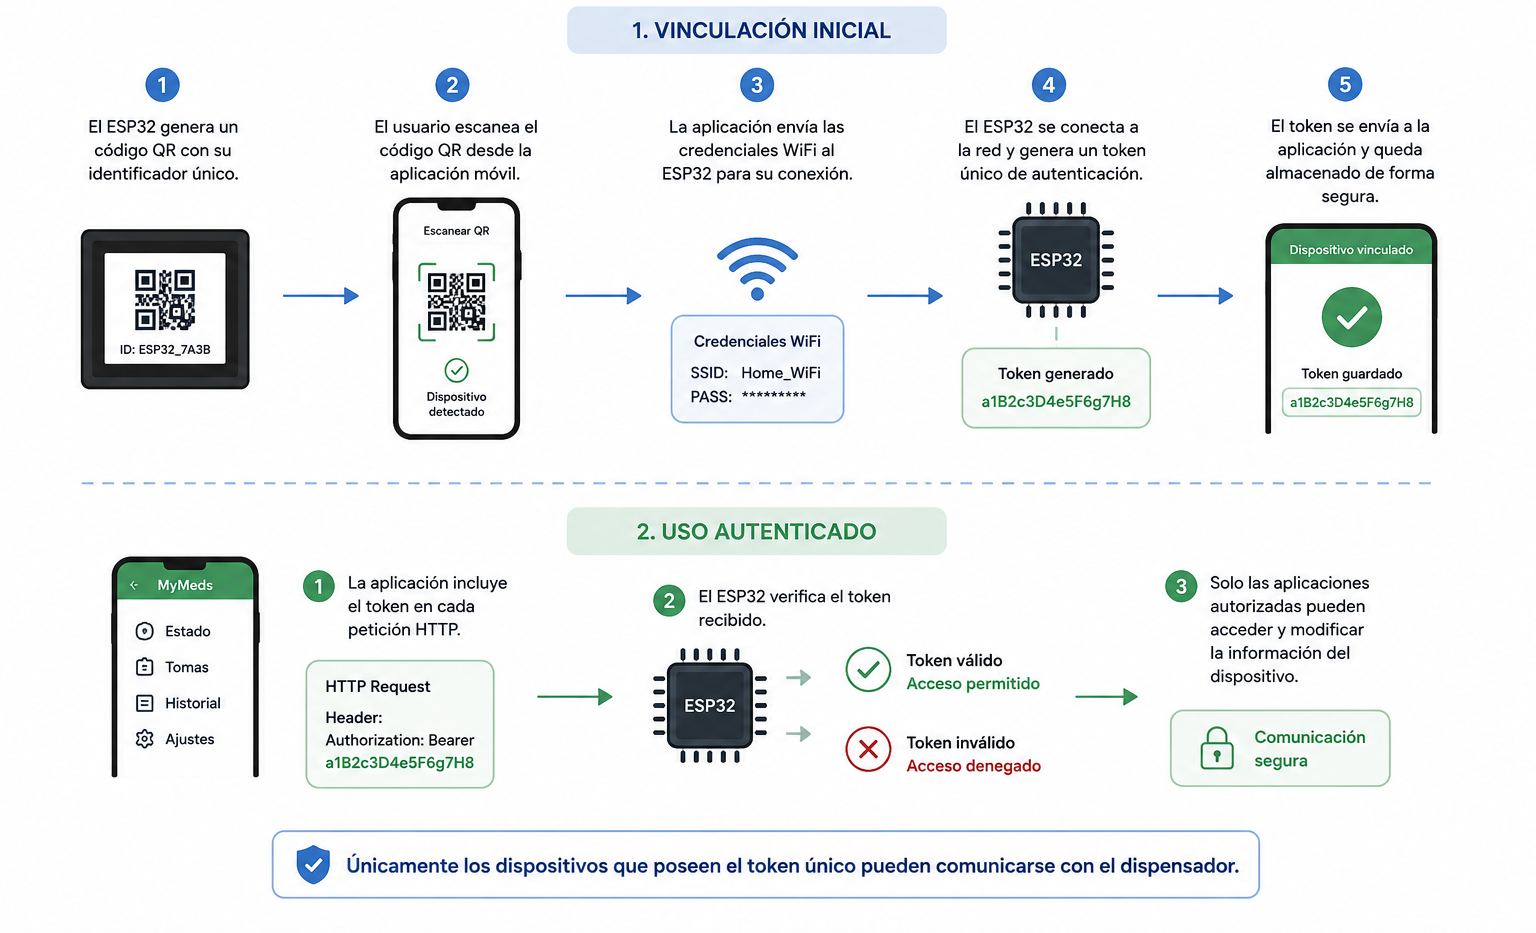
\includegraphics[width=0.96\textwidth]{figs/autenticacion.png}
\caption{[Elaboración propia con IA]}
\end{center}

\note[item]{
\item PIN
\item Token sesión
\item Autorización
\item Protección WiFi
\item Validación
}

\end{frame}

\begin{frame}
\frametitle{Validación experimental de la seguridad}

\begin{center}
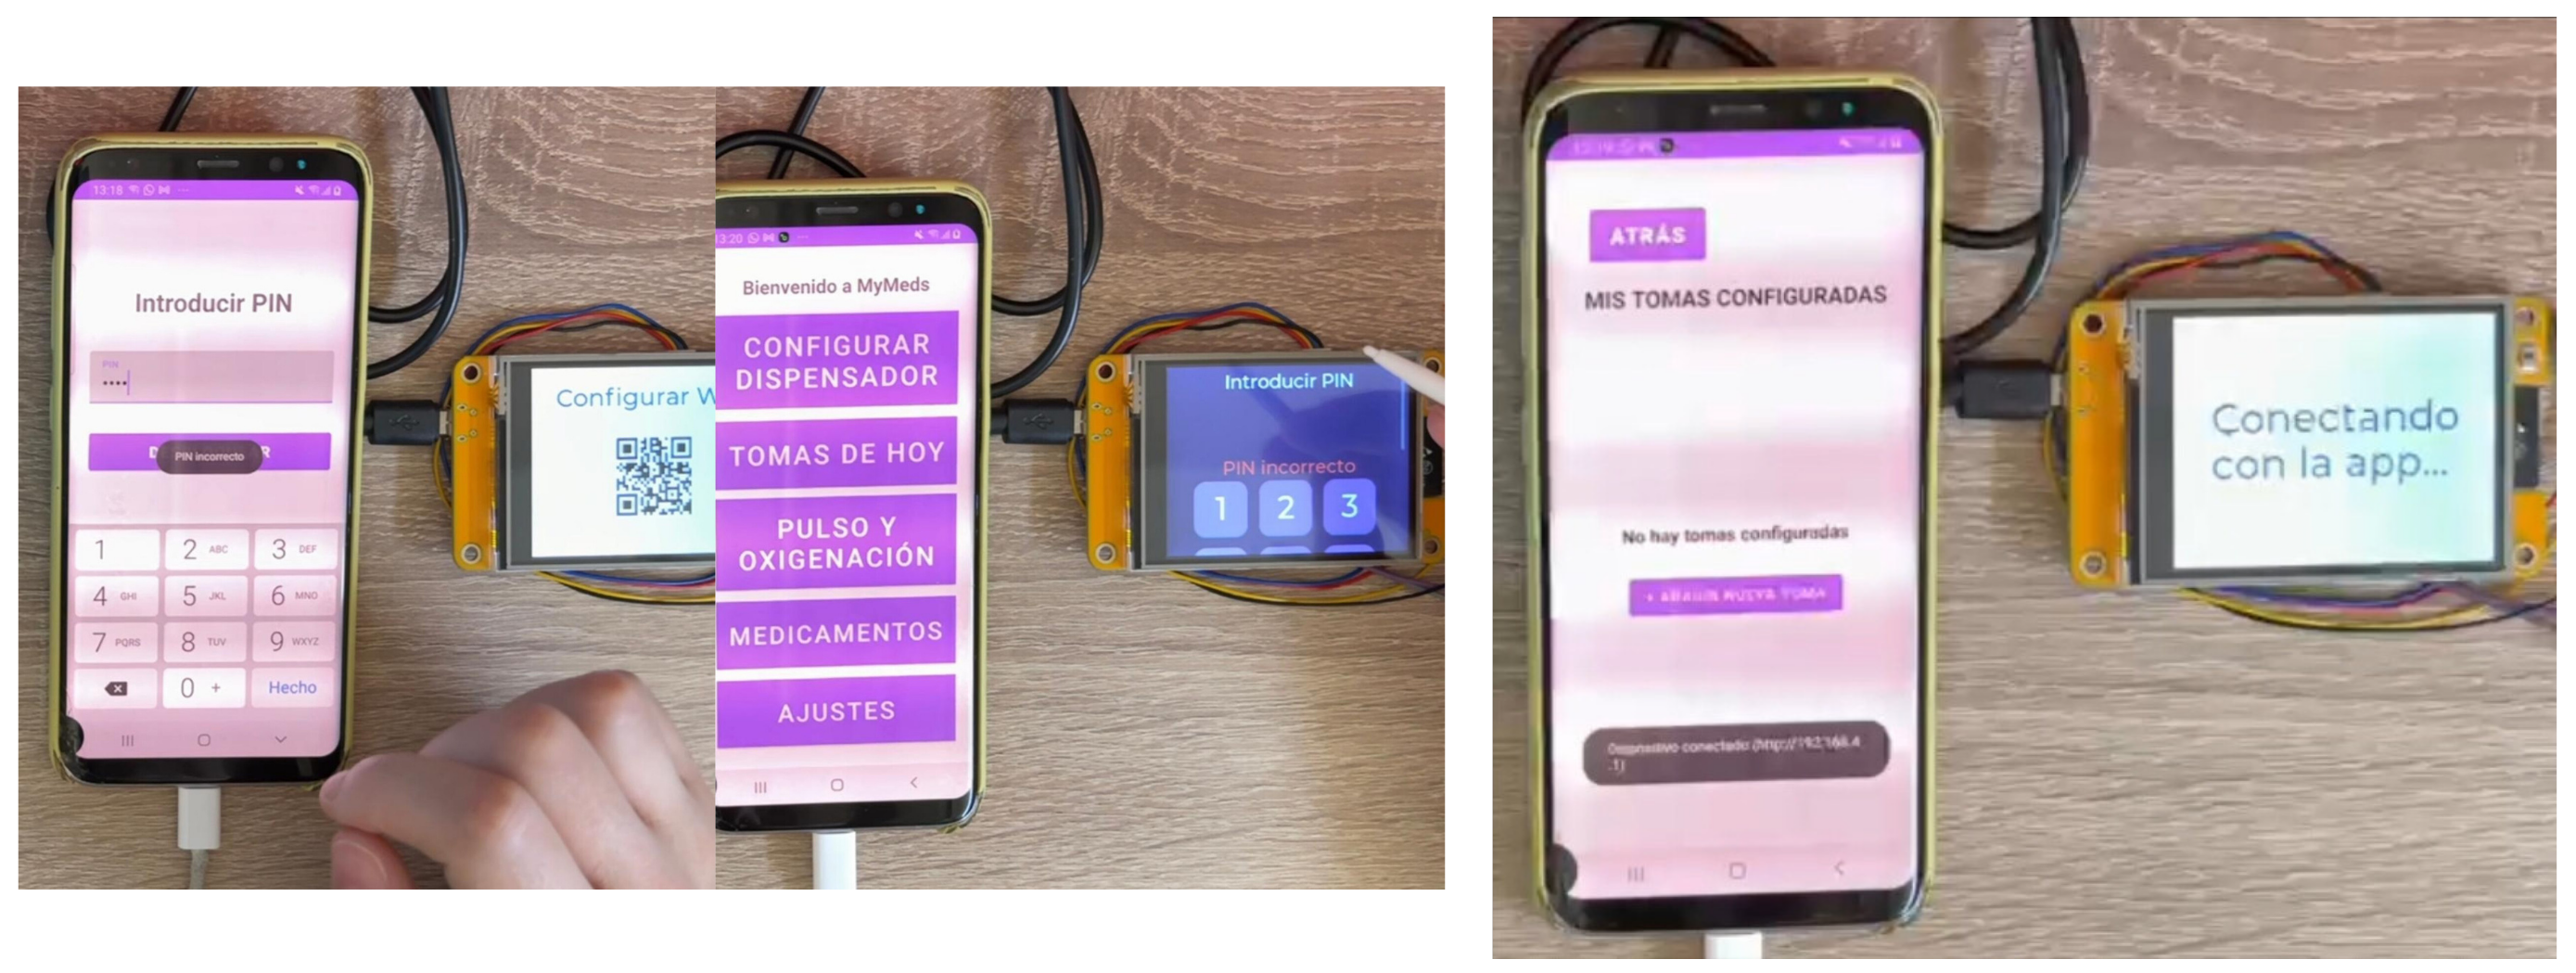
\includegraphics[width=\textwidth]{figs/experimentos_seguridad.png}
\end{center}

\note[item]{
\item PIN correcto
\item Token generado
\item Acceso permitido
\item PIN incorrecto
\item Acceso denegado
\item Validación completa
\item Conclusiones
}

\end{frame}

\begin{frame}
\frametitle{Validación experimental de la seguridad}

\begin{center}
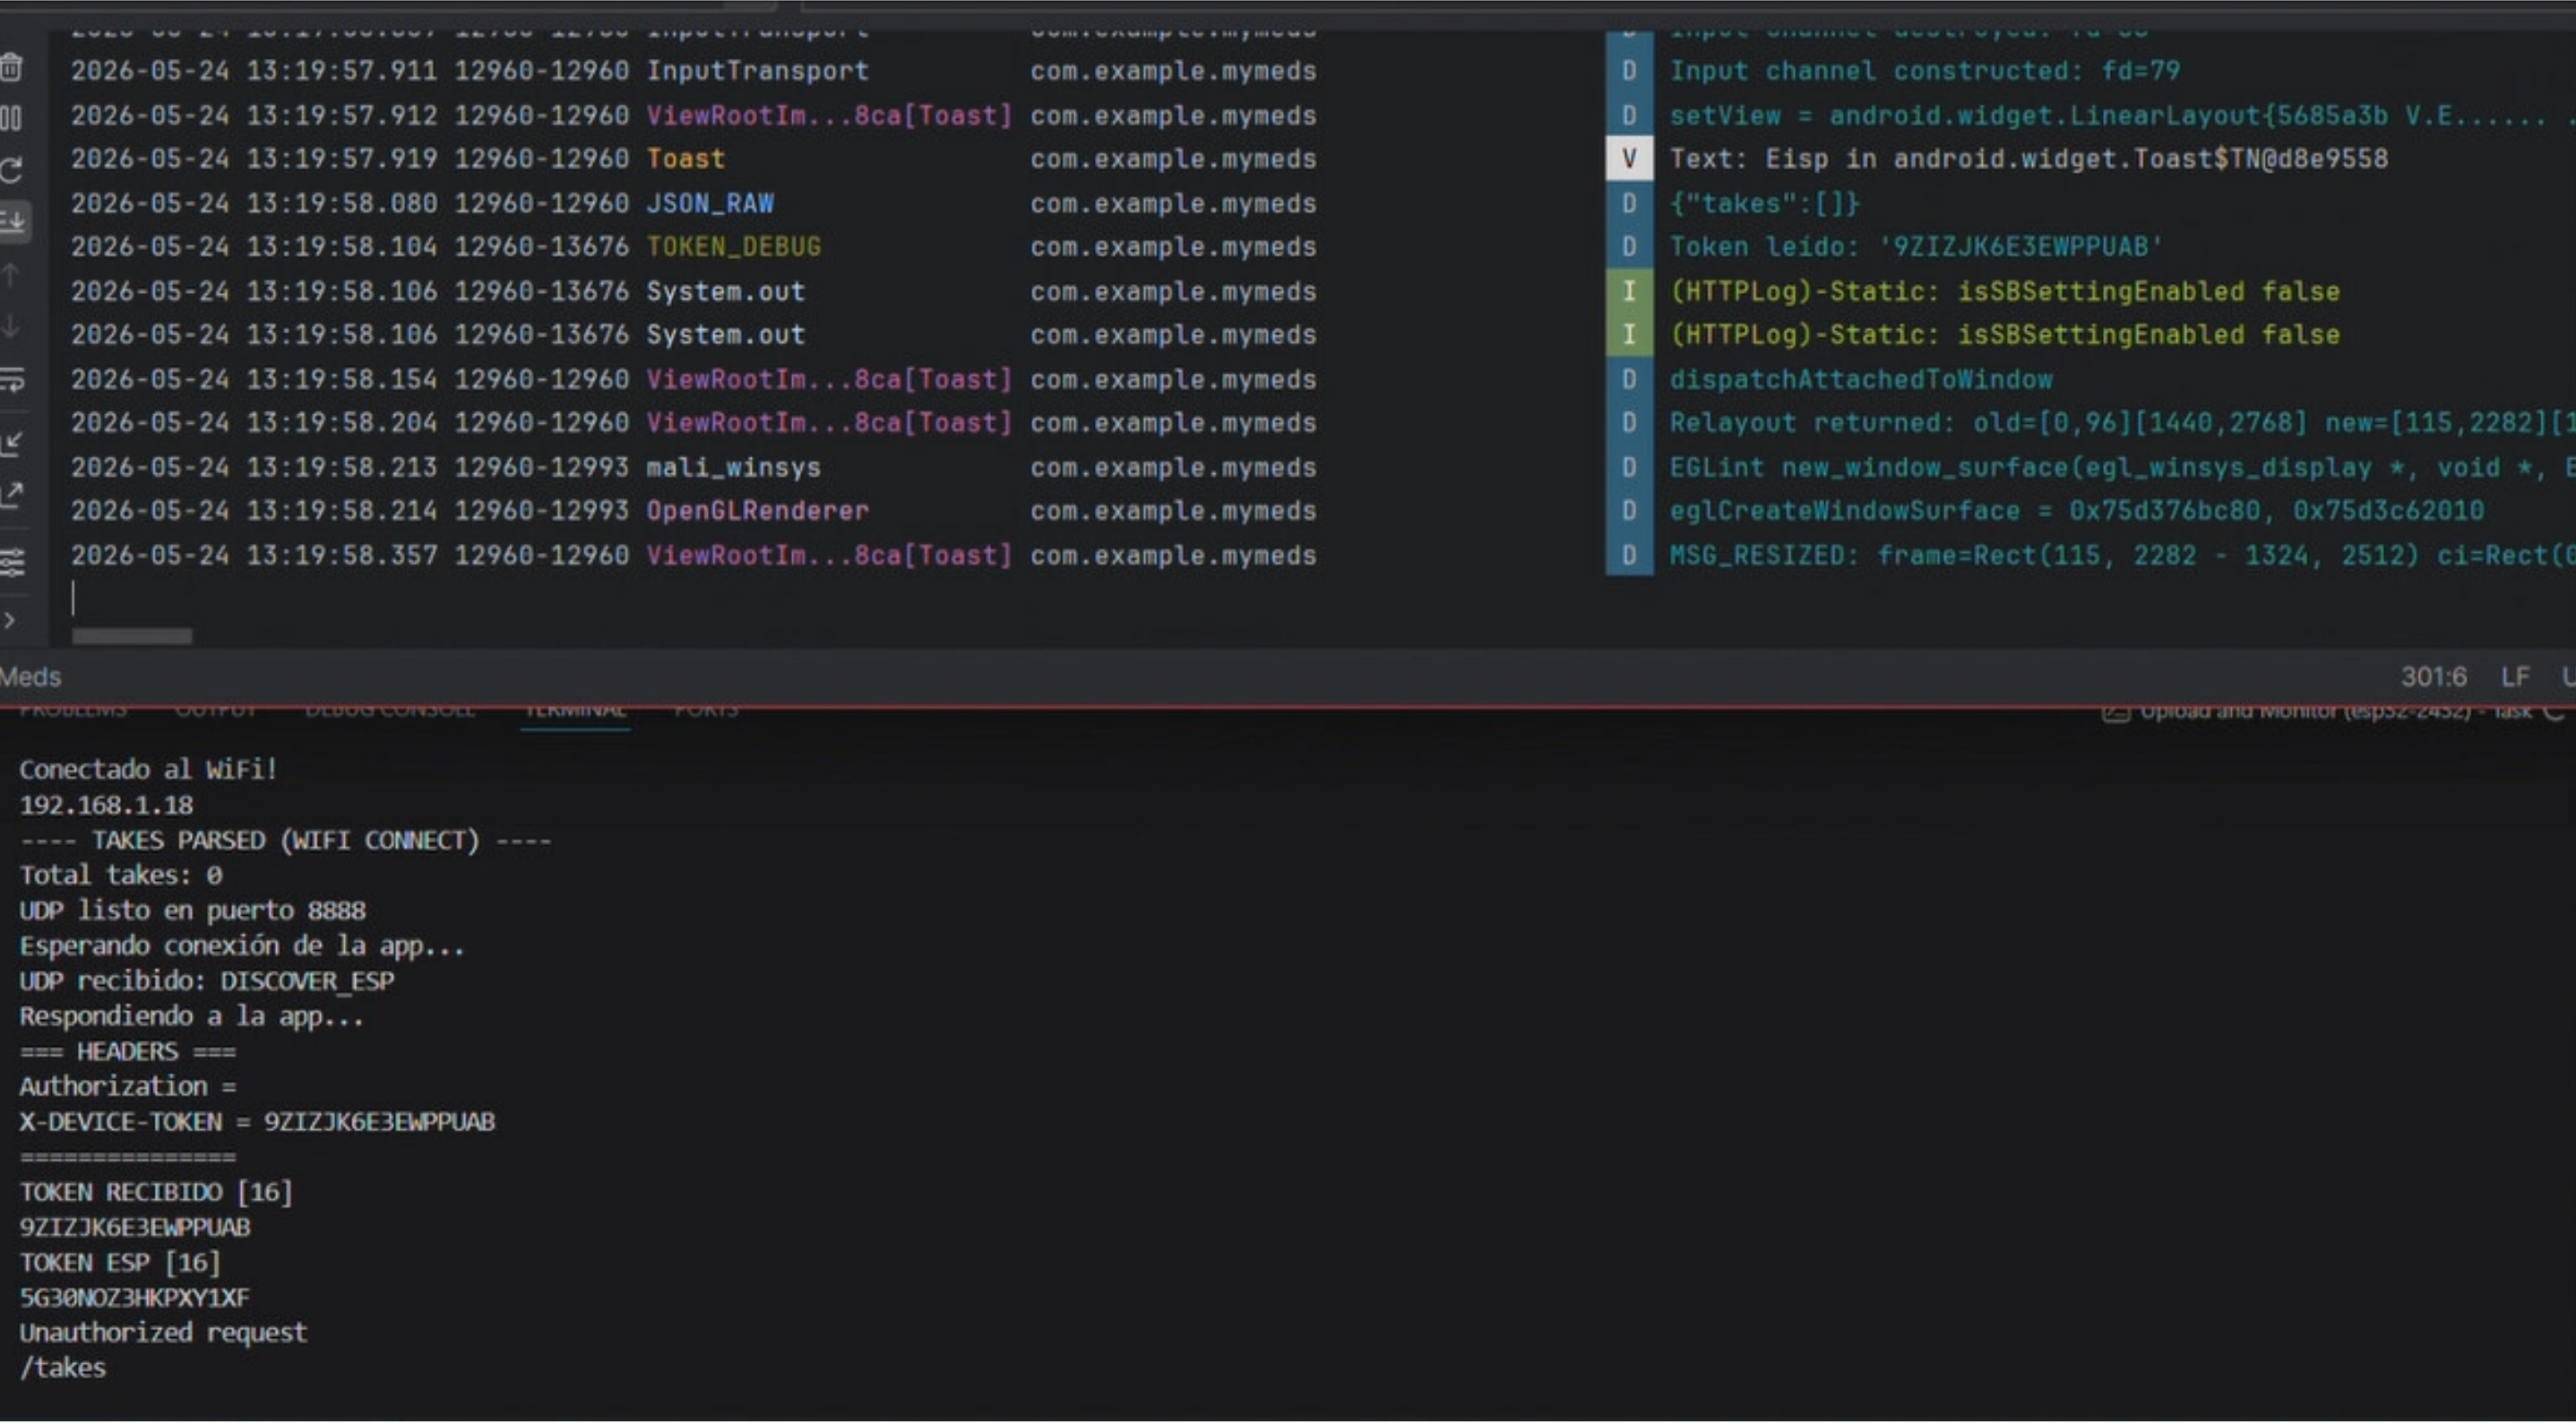
\includegraphics[width=\textwidth]{figs/terminal_seguridad.png}
\end{center}

\note[item]{
Tras generar el token de autenticación, se comprobó que únicamente las peticiones que incluían un token válido eran aceptadas por el servidor del dispositivo.
}

\end{frame}

%==================================================
\section*{}
\begin{frame}{}
  \centering \Huge
  \emph{Conclusiones}
  \note[item]{Para finalizar, me gustaría destacar las principales conclusiones obtenidas tras el desarrollo de este trabajo.}
\end{frame}

\section{Conclusiones}
\subsection{Objetivos alcanzados}

\begin{frame}
\begin{block}{Objetivos alcanzados}
\begin{itemize}
\item Desarrollo de un \textcolor{red}{dispensador inteligente} para el entorno doméstico.
\item Integración de \textcolor{red}{hardware y software} en un único sistema.
\item Desarrollo de una \textcolor{red}{aplicación Android} para gestión remota.
\item Integración de \textcolor{red}{monitorización biomédica} con el sensor MAX30102.
\item \textcolor{red}{Validación experimental} del funcionamiento del sistema.
\end{itemize}
\end{block}

\vspace{0.3cm}

\begin{block}{Resultado final}
\centering
\textcolor{red}{MyMeds constituye un prototipo funcional de asistencia sanitaria doméstica de bajo coste.}
\end{block}

\note[item]{
\item MyMeds desarrollado
\item HW + SW
\item Firmware + App
\item Validación completa
\item Objetivos cumplidos
\item Sistema funcional
\item Bajo coste
\item Líneas futuras
}

\end{frame}

\subsection{Líneas futuras}
\begin{frame}

\begin{block}{Líneas futuras}
\begin{itemize}
\item Integración con \textcolor{red}{sistemas sanitarios}.
\item Soporte \textcolor{red}{multiusuario}.
\item Integración de nuevos \textcolor{red}{sensores biomédicos}.
\item \textcolor{red}{Notificaciones remotas} para cuidadores.
\item Aplicación de \textcolor{red}{inteligencia artificial}.
\end{itemize}
\end{block}

\vspace{0.3cm}

\begin{block}{Perspectiva}
\centering
\textcolor{red}{Estas mejoras permitirían evolucionar MyMeds hacia una solución más completa, escalable y preparada para entornos reales.}
\end{block}

\note[item]{
\item Historia clínica
\item Multiusuario
\item Nuevos sensores
\item Notificaciones
\item IA
}

\end{frame}
% %========= Diapositiva "vacía" de comienzo de sección:
% \section*{}
% \begin{frame}{}
%   \centering \Huge
%   \emph{Introducción}
% \note[item]{Comencemos con la introducción.}
% \end{frame}
%
% \section{Introducción}
% \subsection{Contexto general}
% %========= Diapositiva con imágenes:
% \begin{frame}
% \frametitle{Situación de la Robótica}
% \begin{figure}
% \centering
% 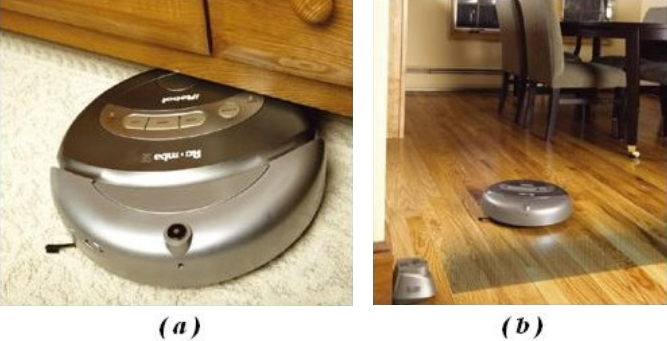
\includegraphics[width=3.4cm]{figs/roomba.jpg}
% \end{figure}
% \end{frame}
%
% %========= Diapositiva con ítems resaltados con colores:
% \begin{frame}
% \frametitle{Situación de la Robótica}
% \begin{itemize}
% \item La \textcolor{red}{tecnología} está cada vez más presente en la vida cotidiana.
% \item Los robots de servicio aparecen en el \textcolor{blue}{mercado}.
% \item La \textcolor{red}{domótica} presenta cada vez más aplicaciones domésticas.
% \end{itemize}
% \end{frame}
%
% \subsection{Contexto específico}
% %========= Diapositiva con bloques:
% \begin{frame}
% \frametitle{Precedentes de la robótica}
% \begin{block}{Primera revolución industrial de 1800}
% Productos fabricados por \textcolor{blue}{máquinas}. La \textcolor{red}{máquina de vapor} fue clave.
% \end{block}
% \end{frame}
%
% %========= Diapositiva con bullets en diferentes niveles (outline):
% \section{Principios de transducción}
% \subsection{Principio de transducción piezoresistivo}
% \begin{frame}
% \frametitle{Conceptos}
% \begin{outline}
% \1 Piezoresistividad: relación entre resistencia eléctrica y deformación.
% \2 Material piezoresistivo: (1) material en reposo (átomos en equilibrio).
% \3 (2) Si sufre deformación, movimiento átomos, modifican su resistividad.
% \2 Resistencia vs. resistividad de un material.
% \3 Resistencia: depende del volumen del material a tratar.
% \3 Resistividad: caract. intrínseca relacionada con colocación de átomos.
% \end{outline}
% \end{frame}
%
% \section*{}
% \begin{frame}{}
%   \centering \Huge
%   \emph{Objetivos}
% \note[item]{Pasemos ahora a comentar los objetivos que nos hemos con este trabajo.}
% \end{frame}
%
% \section{Objetivos}
% \begin{frame}
% \begin{enumerate}
% \item Crear una herramienta multiplataforma.
% \item Sin necesidad de instalación.
% \item Toda ejecución vía web.
% \end{enumerate}
% \end{frame}
%
% \section*{}
% \begin{frame}{}
%   \centering \Huge
%   \emph{Diseño}
% \note[item]{Una vez descritos los objetivos, veamos qué hemos hecho para alcanzarlos.}
% \end{frame}
%
% \section{Diseño}
% %========= Diapositiva con matemáticas:
% \subsection{Matemáticas empleadas}
% \begin{frame}
% \frametitle{Matrices de la cámara}
% \begin{itemize}
% \item Se usa una matriz $RT (4x4)$ en lugar de $R$ y $T$.
% \item La matriz $RT$ rota $\theta$ grados en los ejes $X$, $Y$ y $Z$:
% \end{itemize}
% \begin{equation}
% 	\begin{bmatrix}
% 	1 & 0 & 0 & X \\
% 	0 & cos(\theta) & sin(\theta) &	Y \\
% 	0 & -sin(\theta)& cos(\theta) & Z \\
% 	0 & 0 & 0 & 1
% 	\end{bmatrix}
% \end{equation}
% \end{frame}
%
% %========= Diapositiva con matemáticas y leyenda (conditions*):
% \begin{frame}
% \frametitle{Resistencia de un material}
% \begin{outline}
% \1 Si material piezoresistivo se deforma, cambia su resistencia eléctrica.
% \begin{equation}
% R=\rho\frac{l}{A}
% \end{equation}
% donde:
% \begin{conditions*}
% R & resistencia del material $[\Omega]$\\
% \rho & resistividad $[\Omega-m]$\\
% l & longitud $[m]$\\
% A & área de sección transversal $[m^2]$
% \end{conditions*}
% \1 El cambio de resistencia se obtiene a partir de:
% \begin{equation}
% \frac{\Delta R}{R}=\frac{\Delta\rho}{\rho}=\frac{\Delta A}{A}=\frac{\Delta l}{l}
% \end{equation}
% \1 Otra forma de medir el efecto piezoresistivo: el factor de deformación.
% \begin{equation}
% GF(\textit{Gauge Factor})=\frac{\frac{\Delta R}{R}}{\varepsilon}=\frac{\frac{\Delta R}{R}}{\frac{\Delta l}{l}}
% \end{equation}
% \end{outline}
% \end{frame}
%
% %========= Diapositiva con códigos:
% \subsection{Algoritmo principal}
% \begin{frame}[fragile]
% \frametitle{Algoritmo de visión}
% \begin{lstlisting}
% cvCvtColor (&image, IplTmp1, CV_RGB2GRAY);//to Gray
% cvNormalize(IplTmp1, IplTmp1, 0, 255, CV_MINMAX);
% cvSmooth(IplTmp1,IplTmp2,CV_BLUR,3,3);//Avrg filter
% cvLaplace(IplTmp2, IplLaplace, 3);//Laplace
% cvConvertScale(IplLaplace,IplTmp1);
% cvThreshold(IplTmp1,IplTmp2,Thress,255,CV_THRESH_BIN);
% \end{lstlisting}
% \end{frame}
%
% \section*{}
% \begin{frame}{}
%   \centering \Huge
%   \emph{Conclusiones}
% \note[item]{Para acabar esta presentación, vamos a repasar lo hecho, unas breves conclusiones y las líneas futuras.}
% \end{frame}

\begin{frame}[plain]
\large{\titlepage}
\note[item]{
Hasta aquí mi presentación, y ahora, con el permiso del tribunal, voy a dedicar unos minutos a hacer una pequeña demo en vivo.}
\end{frame}

\end{document}
